%%%%%%%%%%%%%%%%%%%%%%%%%%%%%%%%%%%%%%%%%%%%%%%%%%%%%%%%%%%%%%%%%%%%%%%%%%%%%%%%%%%%%
%%%%%%%%%          DOCUMENTO DE UNION DE CAPITULOS                      %%%%%%%%%%%%%
%%%%%%%%%%%%%%%%%%%%%%%%%%%%%%%%%%%%%%%%%%%%%%%%%%%%%%%%%%%%%%%%%%%%%%%%%%%%%%%%%%%%%
%\documentclass[12pt,oneside,a4paper]{book}
\documentclass[twoside,12pt, pdftex]{classes/CUEDthesisPSnPDF}
%{classes/CUEDthesisPSnPDF}

\usepackage{ae}
\usepackage[spanish]{babel}
\selectlanguage{spanish}
\usepackage[OT2,T1]{fontenc}
\usepackage{times}							%%% Uso de letra Time
\usepackage[utf8]{inputenc}				%%% Este paquete permite poner acentos directamente%%% 
\usepackage[pdftex]{graphicx,color}			%%% Inclusion de Figuras 
\usepackage{titlesec}
\usepackage{fancyhdr}
\usepackage{hyperref}
\usepackage{makeidx}
\usepackage{tocbibind}
\usepackage[intlimits]{amsmath}
\usepackage{cancel}
\usepackage{listings}
\usepackage[usenames,dvipsnames]{color}
\usepackage[final]{stylefiles/mcode}
\usepackage{enumerate}
\usepackage{wasysym}
\usepackage{caption}
\usepackage{subcaption}

%%%%%%%%%%%%%%% Formato de capítulos %%%%%%%%%%%%%%%%%%%%%
\newcommand{\sublinea}{\titlerule[.3mm] \vspace{.5mm} \titlerule[.75mm]}%
\titleformat{\chapter}[display] %%% definicion a cambiar % 
{\bfseries \sffamily \huge}%%% tipo de letra y tamao     % 
{\filleft                                                % 
 \LARGE \chaptertitlename\ %%% tamao Large               % 
 \Huge \thechapter}%%% n en Large                        % 
{3mm}%%% espacio entre etiqueta y cuerpo                 %
{\filleft}                                               %
[\vspace{0.5mm} \sublinea]                               % 
%%%%%%%%%%%%%%%%%%%%%%%%%%%%%%%%%%%%%%%%%%%%%%%%%%%%%%%%%%

%%%%%%%%%%%%%%% configuracin de pgina %%%%%%%%%%%%%%%%%%
\addtolength{\hoffset}{-5pt}                             %  
\addtolength{\voffset}{-25pt}                            %  
\addtolength{\textwidth}{50pt}                           %
\addtolength{\headheight}{12pt}                          % 
\addtolength{\textheight}{75pt}                          %  
%%%%%%%%%%%%%%%%%%%%%%%%%%%%%%%%%%%%%%%%%%%%%%%%%%%%%%%%%%

%%%%%%%%%%%%%%%%%%%%%%%%%%%%%%%%%%%%%%%%%%%%%%%%%%%%%%%%%%
%%%%%%%%%%%%%%%%% DEFINICIN DE MACROS %%%%%%%%%%%%%%%%%%%%
%%% MACRO FIGURA 										 %
%%%%%%%%%%%%%%%%%%%%%%%%%%%%%%%%%%%%%%%%%%%%%%%%%%%%%%%%%%
% Comando:                                               %
% \figura{nombre-fichero}{argumentos}{titulo}{etiqueta}  %
% argumnetos: width=Xcm,height=Ycm,angle=z               %  
%%%%%%%%%%%%%%%%%%%%%%%%%%%%%%%%%%%%%%%%%%%%%%%%%%%%%%%%%%
\newcommand{\figura}[4]{                                 %
   \begin{figure}[htbp]                                   %
   	\centering                                           %
	\includegraphics[#2]{#1}                             %
	\caption{\footnotesize#3}                            %
	\label{#4}                                           %
\end{figure}                                             %  
             }                                           %

%%%%%%%%%%%%%%%%%%%%%%%%%%%%%%%%%%%%%%%%%%%%%%%%%%%%%%%%%%

\newcommand{\figu}[4]{                                 %
   \begin{figure}[!hp]                                   %
	\centering                                           %
	\includegraphics[#2]{#1}                             %
	\caption{\footnotesize#3}                            %
	\label{#4}                                           %
\end{figure}                                             %  
             }                                           %
%%%%%%%%%%%%%%%%%%%%%%%%%%%%%%%%%%%%%%%%%%%%%%%%%%%%%%%%%%%
%%%%%%%%%%%%%%%%%%%%%%%%%%%%%%%%%%%%%%%%%%%%%%%%%%%%%%%%%%
% MACRO GRAD (Para colocar el simbolo ° ) % 
%%%%%%%%%%%%%%%%%%%%%%%%%%%%%%%%%%%%%%%%%%%%%%%%%%%%%%%%%%

\newcommand{\grad}{\hspace{-2mm}$\phantom{a}^{\circ}$\hspace{1mm}}

%%%%%%%%%%%%%%%%%%%%%%%%%%%%%%%%%%%%%%%%%%%%%%%%%%%%%%%%%%
% MACRO SUMARIO(SOLO PARA SER USADO DENTRO DE CAPITULOS) % 
%%%%%%%%%%%%%%%%%%%%%%%%%%%%%%%%%%%%%%%%%%%%%%%%%%%%%%%%%%
% Comando:                                               %
% \sumario{nombre de referencia de la seccin}            %
% ********** PARA SECCIONES ***************************  %     
%%%%%%%%%%%%%%%%%%%%%%%%%%%%%%%%%%%%%%%%%%%%%%%%%%%%%%%%%%
\newcommand{\sumario}[1]{                                %
\newline                                                 %
\vspace*{2pt}                                            %
\textsc{\ref{#1} $\circ$ \nameref{#1}}                   %
                          }                              %
%%%%%%%%%%%%%%%%%%%%%%%%%%%%%%%%%%%%%%%%%%%%%%%%%%%%%%%%%%
%%%%%%%%%%%%%%%%%%%%%%%%%%%%%%%%%%%%%%%%%%%%%%%%%%%%%%%%%%
% Comando:                                               %
% \subsumario{nombre de referencia de la subseccin}      %
% ********* PARA SUB-SECCIONES ************************* %
%%%%%%%%%%%%%%%%%%%%%%%%%%%%%%%%%%%%%%%%%%%%%%%%%%%%%%%%%%
\newcommand{\subsumario}[1]{                             %
\newline                                                 %
\vspace*{1pt}                                            %
\hspace*{1cm} {\small - \nameref{#1}}                    %
                          }                              %
%%%%%%%%%%%%%%%%%%%%%%%%%%%%%%%%%%%%%%%%%%%%%%%%%%%%%%%%%%
%%%%%%%%%%%%%%%%%%%%%%%%%%%%%%%%%%%%%%%%%%%%%%%%%%%%%%%%%%
% Comando:                                               %
% \subsumario{nombre de referencia de la subseccin}      %
% ********* PARA SUB-SUB-SECCIONES ********************* %
%%%%%%%%%%%%%%%%%%%%%%%%%%%%%%%%%%%%%%%%%%%%%%%%%%%%%%%%%%
\newcommand{\subsubsumario}[1]{                          %
\newline                                                 %
\vspace*{1pt}                                            %
\hspace*{2cm} {\small   \nameref{#1}}                    %
                          }                              %
%%%%%%%%%%%%%%%%%%%%%%%%%%%%%%%%%%%%%%%%%%%%%%%%%%%%%%%%%%
%%%%%%%%%%%%%%%%%%%%%%%%%%%%%%%%%%%%%%%%%%%%%%%%%%%%%%%%%%
% MACRO ECUACIN                                          % 
%%%%%%%%%%%%%%%%%%%%%%%%%%%%%%%%%%%%%%%%%%%%%%%%%%%%%%%%%%
% Comando:                                               %
% \ecu{etiqueta}{contenido}                              %
%%%%%%%%%%%%%%%%%%%%%%%%%%%%%%%%%%%%%%%%%%%%%%%%%%%%%%%%%%
\newcommand{\ecu}[2]{                                    %
  \begin{equation}                                       %
    #2                                      			 %
    \label{#1}                                           %
  \end{equation}           }                             %
%%%%%%%%%%%%%%%%%%%%%%%%%%%%%%%%%%%%%%%%%%%%%%%%%%%%%%%%%%
%%%%%%%%%%%%%%%%%%%%%%%%%%%%%%%%%%%%%%%%%%%%%%%%%%%%%%%%%%
% Referencia de Figura                                   % 
%%%%%%%%%%%%%%%%%%%%%%%%%%%%%%%%%%%%%%%%%%%%%%%%%%%%%%%%%%
% Comando:                                               %
% \reffig{nombre figura}                                 %
%%%%%%%%%%%%%%%%%%%%%%%%%%%%%%%%%%%%%%%%%%%%%%%%%%%%%%%%%%
\newcommand{\reffig}[1]{                                 %
  \textit{Figura \ref{fig:#1}}                           %
                        }                                %
%%%%%%%%%%%%%%%%%%%%%%%%%%%%%%%%%%%%%%%%%%%%%%%%%%%%%%%%%%
%%%%%%%%%%%%%%%%%%%%%%%%%%%%%%%%%%%%%%%%%%%%%%%%%%%%%%%%%%
% Referencia de anexo                                    % 
%%%%%%%%%%%%%%%%%%%%%%%%%%%%%%%%%%%%%%%%%%%%%%%%%%%%%%%%%%
% Comando:                                               %
% \refanex{nombre anexo}                                %
%%%%%%%%%%%%%%%%%%%%%%%%%%%%%%%%%%%%%%%%%%%%%%%%%%%%%%%%%%
\newcommand{\refanex}[1]{                                %
  \textit{Anexo \ref{#1}}			  			     %
}														 %
%%%%%%%%%%%%%%%%%%%%%%%%%%%%%%%%%%%%%%%%%%%%%%%%%%%%%%%%%%
%%%%%%%%%%%%%%%%%%%%%%%%%%%%%%%%%%%%%%%%%%%%%%%%%%%%%%%%%%
% Referencia de Seccion                                  % 
%%%%%%%%%%%%%%%%%%%%%%%%%%%%%%%%%%%%%%%%%%%%%%%%%%%%%%%%%%
% Comando:                                               %
% \refsec{nombre seccion}                                %
%%%%%%%%%%%%%%%%%%%%%%%%%%%%%%%%%%%%%%%%%%%%%%%%%%%%%%%%%%
\newcommand{\refsec}[1]{                                 %
  \textit{Secci\'on \ref{sec:#1}}						 %
}														 %
%%%%%%%%%%%%%%%%%%%%%%%%%%%%%%%%%%%%%%%%%%%%%%%%%%%%%%%%%%
%%%%%%%%%%%%%%%%%%%%%%%%%%%%%%%%%%%%%%%%%%%%%%%%%%%%%%%%%%
% Referencia de subseccion                               % 
%%%%%%%%%%%%%%%%%%%%%%%%%%%%%%%%%%%%%%%%%%%%%%%%%%%%%%%%%%
% Comando:                                               %
% \refsubsec{nombre subseccion}                          %
%%%%%%%%%%%%%%%%%%%%%%%%%%%%%%%%%%%%%%%%%%%%%%%%%%%%%%%%%%
\newcommand{\refsubsec}[1]{                              %
  \textit{Secci\'on \ref{subsec:#1}}                     %
                        }                                %
%%%%%%%%%%%%%%%%%%%%%%%%%%%%%%%%%%%%%%%%%%%%%%%%%%%%%%%%%%
% Referencia de Capitulo                                 % 
%%%%%%%%%%%%%%%%%%%%%%%%%%%%%%%%%%%%%%%%%%%%%%%%%%%%%%%%%%
% Comando:                                               %
% \refcap{nombre seccion}                                %
%%%%%%%%%%%%%%%%%%%%%%%%%%%%%%%%%%%%%%%%%%%%%%%%%%%%%%%%%%
\newcommand{\refcap}[1]{                                 %
  \textit{Cap\'itulo \ref{#1}}							 %
}														 %
%%%%%%%%%%%%%%%%%%%%%%%%%%%%%%%%%%%%%%%%%%%%%%%%%%%%%%%%%%
% Referencia de Ecuacin                                  % 
%%%%%%%%%%%%%%%%%%%%%%%%%%%%%%%%%%%%%%%%%%%%%%%%%%%%%%%%%%
% Comando:                                               %
% \refecu{nombre ecuaci\'on}                             %
%%%%%%%%%%%%%%%%%%%%%%%%%%%%%%%%%%%%%%%%%%%%%%%%%%%%%%%%%%
\newcommand{\refecu}[1]{                                 %
  \textit{Ec\hspace{1mm}\ref{#1}}                        %
                        }                                %
%%%%%%%%%%%%%%%%%%%%%%%%%%%%%%%%%%%%%%%%%%%%%%%%%%%%%%%%%%
%%%%%%%%%%%%%%%%%%%%%%%%%%%%%%%%%%%%%%%%%%%%%%%%%%%%%%%%%%
% Salto de renglon                                       % 
%%%%%%%%%%%%%%%%%%%%%%%%%%%%%%%%%%%%%%%%%%%%%%%%%%%%%%%%%%
% Comando:                                               %
% \salto                                                 %
%%%%%%%%%%%%%%%%%%%%%%%%%%%%%%%%%%%%%%%%%%%%%%%%%%%%%%%%%%
\newcommand{\salto}{                                     % 
\vspace*{11pt}      }                                    %
%%%%%%%%%%%%%%%%%%%%%%%%%%%%%%%%%%%%%%%%%%%%%%%%%%%%%%%%%%

%%%%%%%%%%%%%%%%%%%%%%%%%%%%%%%%%%%%%%%%%%%%%%%%%%%%%%%%%%
\newcommand{\referencia}[1]{                                  %
  \textit{[\cite{#1}]}                           %
                        }      							 %
%%%%%%%%%%%%%%%%%%%%%%%%%%%%%%%%%%%%%%%%%%%%%%%%%%%%%%%%%%

%%%%%%%%%%%%%%%%%%%%%%%%%%%%%%%%%%%%%%%%%%%%%%%%%%%%%%%%%%
% Unidades: Nanosegundos, micro metros, nanómetros, etc.
%
\newcommand{\ns} {\textrm{ns}}
\newcommand{\nanom} {\textrm{nm}}
\newcommand{\microm} {$\mu\textrm{m}$ }
\newcommand{\mmcuadrado} {$\textrm{mm}^2$}
%
%%%%%%%%%%%%%%%%%%%%%%%%%%%%%%%%%%%%%%%%%%%%%%%%%%%%%%%%%%

% Formato de las letras más cómodos.
\newcommand{\negrita}[1]{\textbf{#1}}
\newcommand{\cursi}[1]{\emph{#1}}
\newcommand{\layout}{\emph{layout }}
\newcommand{\netlist}{\emph{netlist }}

% Includes a MATLAB script.
% The first parameter is the label, which also is the name of the script
%   without the .m.
% The second parameter is the optional caption.
\newcommand{\matlabscript}[2]
  {\begin{itemize}\item[]\lstinputlisting[caption=#2,label=#1]{#1.m}\end{itemize}}


\ifpdf
    \pdfinfo { /Title  (Diseño de un Sumador Rápido en tecnología CMOS utilizando Herramientas de Software Libre)
               /Creator (TeX)
               /Producer (pdfTeX)
               /Author (Leandro Marsó)
               /CreationDate (D:20130606000000)  %format D:YYYYMMDDhhmmss
               /ModDate (D:20131014000000)
               /Subject (Diseño de Circuitos Integrados)
               /Keywords (Circuitos Integrados VLSI Sumador Rápido)}
    
\fi


%\makeindex \label{indice}

\begin{document}
\sloppy

\begin{titlepage}
\pagestyle{empty}       

\begin{center}
	\Huge{Universidad Nacional de Córdoba\\}
	\Large {Facultad de Ciencias Exáctas, Físicas y Naturales}\\

\vspace{1cm}

%	
\includegraphics[width=50mm]{tapa/dibujo.pdf}\\

\includegraphics{tapa/escudo2.pdf}


\vspace{1cm}

%	\textbf{\Large{Marxismo y Feminismo}}\\%[2ex]
%	\large{ ``Textos seleccionados'' }\\

	\Huge \textbf{\\[2ex]Proyecto Integrador}
	\Large \textsl{\\[2ex] '' Diseño de un Sumador Rápido y de Bajo Consumo en tecnología CMOS submicrónica utilizando Herramientas de Software Libre''}

%\begin{flushright}
	\begin{normalsize}
%		\\Compilación de la Cátedra Che Guevara Córdoba 2012}
	\end{normalsize}
	\begin{large}	
		\\ \textbf{Setiembre 2013}
	\end{large}

\end{center}
%\end{flushright}

\vspace{0.5cm}

\begin{center}

%	
\includegraphics[width=50mm]{tapa/escudo2.pdf}
%		\textsl{\\En la Construcción de un Movimiento Político }
%		\\ \uri{http://cordobasemueve.org.ar}


\end{center}

% turn of those nasty overfull and underfull hboxes
\hbadness=10000
\hfuzz=50pt
\end{titlepage}
			%%% INCLUYE DE CARATULA 
\maketitle

%\frontmatter
%% Copyright 2007 by Till Tantau
%
% This file may be distributed and/or modified
%
% 1. under the LaTeX Project Public License and/or
% 2. under the GNU Public License.
%
% See the file doc/licenses/LICENSE for more details.
%%%%%%%%%%%%%%%%%%%%%%%%%%%%%%%%%%%%%%%%%%%%%%%%%%%%%%%%%%
% Unidades: Nanosegundos, micro metros, nan�metros, etc.
%
\newcommand{\ns} {\textrm{ns}}
\newcommand{\nanom} {\textrm{nm}}
\newcommand{\microm} {$\mu\textrm{m}$ }
\newcommand{\micromcuadrado} {$\mu\textrm{m}^2$}
\newcommand{\mmcuadrado} {$\textrm{mm}^2$}

%
%%%%%%%%%%%%%%%%%%%%%%%%%%%%%%%%%%%%%%%%%%%%%%%%%%%%%%%%%%

% Formato de las letras m�s c�modos.
\newcommand{\negrita}[1]{\textbf{#1}}
\newcommand{\cursi}[1]{\emph{#1}}
\newcommand{\layout}{\emph{layout }}
\newcommand{\netlist}{\emph{netlist }}




\documentclass{beamer}

%
% DO NOT USE THIS FILE AS A TEMPLATE FOR YOUR OWN TALKS�!!
%
% Use a file in the directory solutions instead.
% They are much better suited.
%


% Setup appearance:

\usetheme{Darmstadt}
\usefonttheme[onlylarge]{structurebold}
\setbeamerfont*{frametitle}{size=\normalsize,series=\bfseries}
\setbeamertemplate{navigation symbols}{}
\setbeamercovered{transparent}

% Standard packages

\usepackage[spanish]{babel}
\usepackage[latin1]{inputenc}
\usepackage{times}
\usepackage[T1]{fontenc}
\usepackage{booktabs}
\usepackage[gen]{eurosym}
\usepackage{subcaption}
%\usepackage{caption}
\usepackage{wasysym}
\usepackage{listings}
\lstset{%                       % Configuraci�n de par�metros de listing.
  basicstyle=\small\ttfamily,     % C�digos con fuente TrueType.
  breaklines=false,                % Rompe l�neas demasiado largas.
  xrightmargin=1cm,               % Margen derecho.
  %escapeinside=wz,                % Para escapar a LaTeX.
}%

% Setup TikZ

\usepackage{tikz}
\usetikzlibrary{arrows}
\tikzstyle{block}=[draw opacity=0.7,line width=1.4cm]


% Author, Title, etc.

\title[Dise�o de circuitos integrados con Software Libre]
{%
  Dise�o de un Sumador R�pido en tecnolog�a CMOS
  submicr�nica utilizando Herramientas de Software Libre
}

\author[Mars�]
{
  Leandro~Mars�\inst{1} \and
  Pablo~Cayuela~(Director)\inst{2} \and
  Hugo~Carrer~(Codirector)\inst{1} 
}

\institute[UNC and others]
{
  \inst{1}%
  Universidad Nacional de C�rdoba, Argentina
  \and
  \vskip-2mm
  \inst{2}%
  Universidad Tecnol�gica Nacional, FRC, Argentina
  \and
  \vskip-2mm
}

\date[FCEFyN 2006]
{Facultad de Ciencias Ex�ctas, F�sicas y Naturales, 2015}

% Delete this, if you do not want the table of contents to pop up at
% the beginning of each subsection:
\AtBeginSubsection[]
{
    \begin{frame}<beamer>{Temario}
          \tableofcontents[currentsection,currentsubsection]
	    \end{frame}
	  }

% The main document

\begin{document}

\begin{frame}
  \titlepage
\end{frame}

\begin{frame}{Temario}
  \tableofcontents
\end{frame}


\section{Introducci�n}
\subsection{Definiciones generales}
\begin{frame}{�Qu� es un sumador r�pido?}

\end{frame}
%-------------------------------------------------------------
\begin{frame}{�Qu� es un circuito integrado?}
  \begin{figure}
  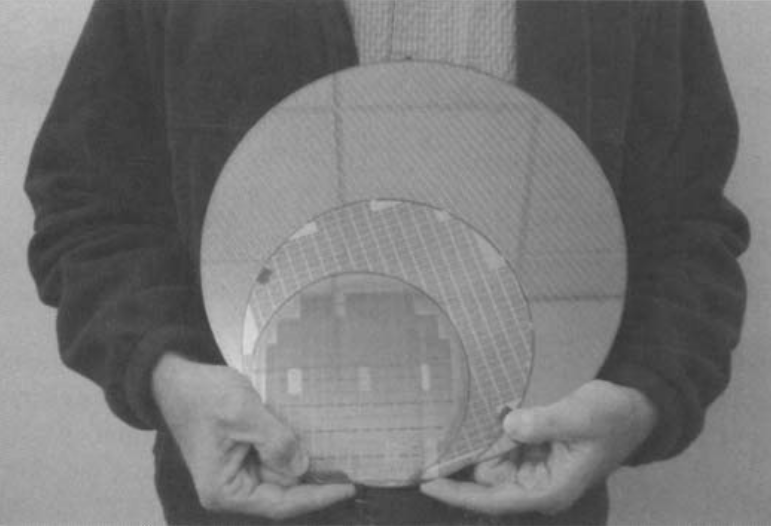
\includegraphics[scale=0.30]{figuras/wafers.png}
  \caption{Obleas de silicio de 150, 200 y 300~mm de d�ametro, de un proceso CMOS.}
  \end{figure}
\end{frame}
%-------------------------------------------------------------
\begin{frame}{�Qu� es un circuito integrado?}
  \begin{figure}
  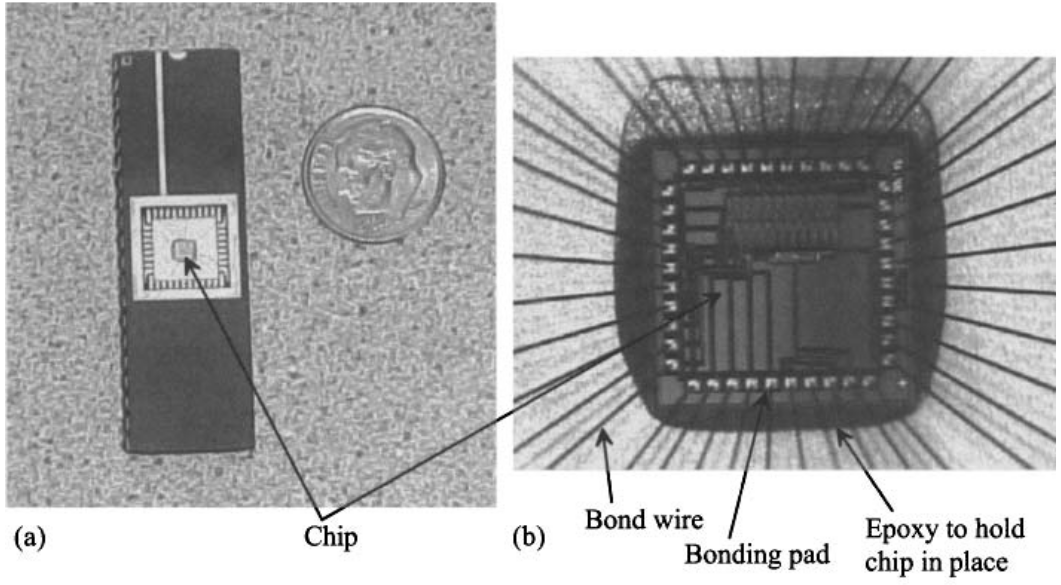
\includegraphics[scale=0.27]{figuras/encapsulado.png}
  \caption{Encapsulado del chip (a) y (b) una vista aumentada.}
  \end{figure}
\end{frame}
%-------------------------------------------------------------
\begin{frame}{�Qu� es un circuito integrado?}
  \begin{figure}
  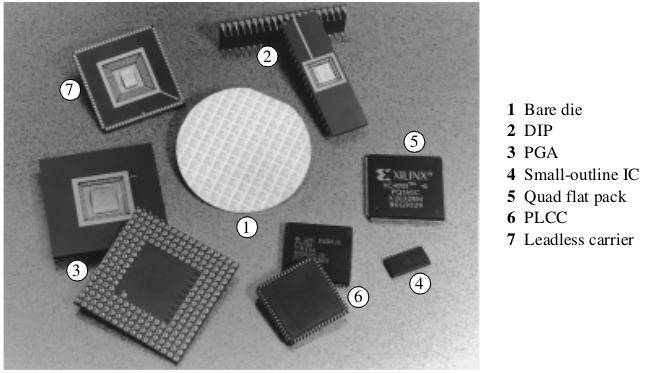
\includegraphics[scale=0.45]{figuras/chips.png}
\caption{Algunos tipos de encapsulados comunes.}
  \end{figure}
\end{frame}
%-------------------------------------------------------------
\begin{frame}{�Qu� es un circuito integrado?}
  \begin{Large}
  \begin{center}
    \textbf{
  �C�mo accedemos a fabricar circuitos integrados?
}
\end{center}
\end{Large}

    \begin{table}[h]
      \centering
      \begin{tabular}{@{}lc@{}}
	\toprule
	\textbf{Fabrica}             & \textbf{Proceso CMOS} \\ \midrule
	TSMC                & 28~nm - 180~nm             \\
	Globalfoundries     & 14~nm - 180~nm             \\
	IBM                 & 32~nm -  250nm            \\
	ON Semi             & 0.35~um - 0.7~um           \\
	Austria Micro Systems & 180~nm - 0.35~um           \\ \bottomrule
      \end{tabular}
      \caption{Procesos disponibles por medio de MOSIS}
      \label{tab:procesosMOSIS}
    \end{table}
\end{frame}
%-------------------------------------------------------------
\begin{frame}{�Qu� es un circuito integrado?}
  \begin{Large}
  \begin{center}
    \textbf{
  �C�mo accedemos a fabricar circuitos integrados?
}
\end{center}
\end{Large}
    \begin{table}[h]
      \centering
      \begin{tabular}{@{}lc@{}}
	\toprule
	\textbf{Fabrica}             & \textbf{Proceso CMOS} \\ \midrule
	STMicroelectronics  & 28~nm - 130~nm             \\
	Austria Micro Systems & 180~nm - 0.35~um           \\ \bottomrule
      \end{tabular}
      \caption{Procesos disponibles por medio de CMP}
      \label{tab:procesosCMP}
    \end{table}

\end{frame}

%-------------------------------------------------------------
\begin{frame}{�Qu� es un circuito integrado?}
  \begin{Large}
  \begin{center}
    \textbf{
  �Cu�nto podemos integrar?
}
\end{center}
\end{Large}

  \begin{columns}[t]
    \column{.43\textwidth}
    \begin{exampleblock}{CMOS 350~nm de AMS}
    \begin{itemize}
      \item 18kGates/mm$^2$
      \item 650~\euro{}/mm$^2$
      \item �rea m�nima 3~mm$^2$
      \item 25 chips
    \end{itemize}
    \end{exampleblock}
    \column{.43\textwidth}
    \begin{exampleblock}{CMOS 180~nm de AMS}
      
    \begin{itemize}
      \item 118~kGates/mm$^2$
      \item 1200~\euro{}/mm$^2$
      \item �rea m�nima 5~mm$^2$
      \item 25 chips
    \end{itemize}
\end{exampleblock}
    \end{columns}
\end{frame}

%-------------------------------------------------------------
\begin{frame}[label=libertades]{�Qu� es el Software Libre?}
\begin{definition}
  �Software libre� es el software que respeta la libertad de los usuarios y la comunidad. A grandes rasgos, significa que los usuarios tienen la libertad de ejecutar, copiar, distribuir, estudiar, modificar y mejorar el software. Es decir, el �software libre� es una cuesti�n de libertad, no de precio.
\end{definition}
\end{frame}
%-------------------------------------------------------------

\begin{frame}{Las cuatro libertades del Software Libre}
Un programa es software libre si los usuarios tienen las cuatro libertades esenciales:
\begin{itemize}
\item<1-> La libertad de ejecutar el programa como se desea, con cualquier prop�sito (libertad 0).
\item<2-> La libertad de estudiar c�mo funciona el programa, y cambiarlo para que haga lo que usted quiera (libertad 1). El \alert{acceso al c�digo fuente} es una condici�n necesaria para ello.
\item<3-> La libertad de redistribuir copias para ayudar a su pr�jimo (libertad 2).
\uncover{\item<4-> La libertad de distribuir copias de sus versiones modificadas a terceros (libertad 3). Esto le permite ofrecer a toda la comunidad la oportunidad de beneficiarse de las modificaciones. El \alert{acceso al c�digo fuente} es una condici�n necesaria para ello.
  }
\end{itemize}
\end{frame}

%-------------------------------------------------------------
%\begin{frame}{Las licencias de uso del software y su importancia}
%  \begin{definition}
%  Algo \alert{alerta} o no.
%
%\end{definition}
%  \hyperlink{libertades<2>}{\beamergotobutton{Cuatro libertades}}
%  \hypertarget{return}{}
%\end{frame}
%-------------------------------------------------------------

\subsection{Planteamiento del problema y motivaci�n}

\begin{frame}{�C�mo dise�ar circuitos integrados con herramientas flexibles y accesibles para todo tipo de uso: acad�mico e industrial?}
  \begin{columns}[t]
    \column{.33\textwidth}
    \begin{exampleblock}{Econ�mico}
      $G\colon$
    \end{exampleblock}
    \column{.33\textwidth}
    \begin{exampleblock}{Acad�mico}
      $G\colon$
    \end{exampleblock}

    \column{.33\textwidth}
    \begin{exampleblock}{Otras razones}
      $G\colon$
    \end{exampleblock}
    \end{columns}

\end{frame}
%-------------------------------------------------------------


%\begin{frame}{What is haplotyping and why is it important?}
%  You hopefully know this after the previous three talks\dots
%\end{frame}
%
%\begin{frame}[t]{General formalization of haplotyping.}
%  \begin{block}{Inputs}
%    \begin{itemize}
%    \item A \alert{genotype matrix} $G$.
%    \item The \alert{rows} of the matrix are \alert{taxa / individuals}.
%    \item The \alert{columns} of the matrix are \alert{SNP sites /
%        characters}. 
%    \end{itemize}
%  \end{block}
%  \begin{block}{Outputs}
%    \begin{itemize}
%    \item A \alert{haplotype matrix} $H$.
%    \item Pairs of rows in $H$ \alert{explain} the rows of $G$.
%    \item The haplotypes in $H$ are \alert{biologically plausible}. 
%    \end{itemize}
%  \end{block}
%\end{frame}
%
%
%\begin{frame}[t]{Our formalization of haplotyping.}
%  \begin{block}{Inputs}
%    \begin{itemize}
%    \item A genotype matrix $G$.
%    \item The rows of the matrix are individuals / taxa.
%    \item The columns of the matrix are SNP sites / characters.
%    \item<alert@1->
%      The problem is directed: one haplotype is known.
%    \item<alert@1->
%      The input is biallelic: there are only two homozygous
%      states (0 and 1) and one heterozygous state (2).
%    \end{itemize}
%  \end{block}
%  \begin{block}{Outputs}
%    \begin{itemize}
%    \item A haplotype matrix $H$.
%    \item Pairs of rows in $H$ explain the rows of $G$.
%    \item<alert@1> The haplotypes in $H$ form a perfect phylogeny.
%    \end{itemize}
%  \end{block}
%\end{frame}
%
%
%\begin{frame}{We can do perfect phylogeny haplotyping efficiently, but
%    \dots}
%  \begin{enumerate}
%  \item \alert{Data may be missing.}
%    \begin{itemize}
%    \item This makes the problem NP-complete \dots
%    \item \dots even for very restricted cases.
%    \end{itemize}
%    \textcolor{green!50!black}{Solutions:}
%    \begin{itemize}
%    \item Additional assumption like the rich data hypothesis. 
%    \end{itemize}
%  \item \alert{No perfect phylogeny is possible.}
%    \begin{itemize}
%    \item This can be caused by chromosomal crossing-over effects.
%    \item This can be caused by incorrect data.
%    \item This can be caused by multiple mutations at the same sites.
%    \end{itemize}
%    \textcolor{green!50!black}{Solutions:}
%    \begin{itemize}
%    \item Look for phylogenetic networks.
%    \item Correct data.
%    \item<alert@1->
%       Find blocks where a perfect phylogeny is possible.
%    \end{itemize}
%  \end{enumerate}
%\end{frame}
%
%
%
%\begin{frame}{How blocks help in perfect phylogeny haplotyping.}
%  \begin{enumerate}
%  \item Partition the site set into overlapping contiguous blocks.
%  \item Compute a perfect phylogeny for each block and combine them.
%  \item Use dynamic programming for finding the partition.
%  \end{enumerate}
%
%  \begin{tikzpicture}
%    \useasboundingbox (0,-1) rectangle (10,2);
%    
%    \draw[line width=2mm,dash pattern=on 1mm off 1mm]
%      (0,1) -- (9.99,1) node[midway,above] {Genotype matrix}
%      (0,0.6666) -- (9.99,0.6666)
%      (0,0.3333) -- (9.99,0.3333)
%      (0,0) -- (9.99,0) node[midway,below] {\only<1>{no perfect phylogeny}};
%
%    \begin{scope}[xshift=-.5mm]
%      \only<2->
%      {
%        \draw[red,block]            (0,.5)   -- (3,.5)
%          node[midway,below] {perfect phylogeny};
%      }
%        
%      \only<3->
%      {
%        \draw[green!50!black,block] (2.5,.5)   -- (7,.5)
%          node[pos=0.6,below] {perfect phylogeny};
%      }
%
%      \only<4->
%      {
%        \draw[blue,block]           (6.5,.5) -- (10,.5)
%          node[pos=0.6,below] {perfect phylogeny};
%      }
%    \end{scope}
%  \end{tikzpicture}
%\end{frame}
%
%\begin{frame}{Objective of the integrated approach.}
%  \begin{enumerate}
%  \item Partition the site set into \alert{noncontiguous} blocks. 
%  \item Compute a perfect phylogeny for each block and combine them. 
%  \item<alert@1-> Compute partition while computing perfect
%    phylogenies. 
%  \end{enumerate}
%
%  \begin{tikzpicture}
%    \useasboundingbox (0,-1) rectangle (10,2);
%
%    \draw[line width=2mm,dash pattern=on 1mm off 1mm]
%      (0,1) -- (9.99,1) node[midway,above] {Genotype matrix}
%      (0,0.6666) -- (9.99,0.6666)
%      (0,0.3333) -- (9.99,0.3333)
%      (0,0) -- (9.99,0) node[midway,below] {\only<1>{no perfect phylogeny}};
%
%    \only<2->
%    {
%      \begin{scope}[xshift=-0.5mm]
%        \draw[red,block] (0,.5)   -- (3,.5) 
%          node[midway,below] {perfect phylogeny}
%                         (8,.5) -- (9,.5);
%
%        \draw[green!50!black,block]
%          (3,.5)   -- (6,.5)
%            node[pos=0.6,below] {perfect phylogeny}
%          (6.4,.5)   -- (8,.5)
%          (9,.5) -- (10,.5);
%
%        \draw[blue,block] (6,.5) -- (6.4,.5)
%          node[midway,below=5mm] {perfect phylogeny};
%      \end{scope}
%    }
%  \end{tikzpicture}
%\end{frame}
%
%
%\begin{frame}{The formal computational problem.}
%
%  We are interested in the computational complexity of \\
%  \alert{the function \alert{$\chi_{\operatorname{PP}}$}}:
%  \begin{itemize}
%  \item It gets genotype matrices as input.
%  \item It maps them to a number $k$.
%  \item This number is minimal such that the sites can be
%    covered by $k$ sets, each admitting a perfect phylogeny.
%    \\
%    (We call this a \alert{pp-partition}.)
%  \end{itemize}
%\end{frame}
%
%
%
%\begin{frame}{Finding pp-partitions of haplotype matrices.}
%  We start with a special case:
%  \begin{itemize}
%  \item The inputs $M$ are \alert{already haplotype matrices}.
%  \item The inputs $M$ \alert{do not allow a perfect phylogeny}.
%  \item What is $\chi_{\operatorname{PP}}(M)$?
%  \end{itemize}
%  \begin{example}
%    \begin{columns}
%      \column{.3\textwidth}
%      $M\colon$
%      \footnotesize
%      \begin{tabular}{cccc}
%        0 & 0 & 0 & 1 \\
%        0 & 1 & 0 & 0 \\
%        1 & 0 & 0 & 0 \\
%        0 & 1 & 0 & 0 \\
%        1 & 0 & 0 & 0 \\
%        0 & 1 & 0 & 1 \\
%        1 & 1 & 0 & 0 \\
%        0 & 0 & 1 & 0 \\
%        1 & 0 & 1 & 0
%      \end{tabular}%
%      \only<2>
%      {%
%        \begin{tikzpicture}
%          \useasboundingbox (2.9,0);
%
%          \draw [red, opacity=0.7,line width=1cm] (1.7 ,1.9) -- (1.7 ,-1.7);
%          \draw [blue,opacity=0.7,line width=5mm] (0.85,1.9) -- (0.85,-1.7)
%                                                  (2.55,1.9) -- (2.55,-1.7);
%        \end{tikzpicture}
%      }
%      \column{.6\textwidth}
%      \begin{overprint}
%        \onslide<1>
%        No perfect phylogeny is possible.
%        
%        \onslide<2>
%        \textcolor{blue!70!bg}{Perfect phylogeny}
%        
%        \textcolor{red!70!bg}{Perfect phylogeny}
%        
%        $\chi_{\operatorname{PP}}(M) = 2$.
%        
%      \end{overprint}
%    \end{columns}
%  \end{example}
%\end{frame}
%
%\begin{frame}{Bad news about pp-partitions of haplotype matrices.}
%  \begin{theorem}
%    Finding \alert{optimal pp-partition of haplotype matrices}\\
%    is equivalent to finding \alert{optimal graph colorings}.
%  \end{theorem}
%
%  \begin{proof}[Proof sketch for first direction]
%    \begin{enumerate}
%    \item Let $G$ be a graph.
%    \item Build a matrix with a column for each vertex of $G$.
%    \item For each edge of $G$ add four rows inducing\\the
%      submatrix $\left(
%        \begin{smallmatrix}
%          0 & 0 \\
%          0 & 1 \\
%          1 & 0 \\
%          1 & 1
%        \end{smallmatrix}\right)$.
%    \item The submatrix enforces that the columns lie in different
%      perfect phylogenies. \qedhere  
%    \end{enumerate}
%  \end{proof}
%\end{frame}
%
%\begin{frame}{Implications for pp-partitions of haplotype matrices.}
%  \begin{corollary}
%    If $\chi_{\operatorname{PP}}(M) = 2$ for a haplotype matrix $M$,
%    we can find an optimal pp-partition in polynomial time. 
%  \end{corollary}
%
%  \begin{corollary}
%    Computing $\chi_{\operatorname{PP}}$ for haplotype matrices is
%    \begin{itemize}
%    \item $\operatorname{NP}$-hard,
%    \item not fixed-parameter tractable, unless
%      $\operatorname{P}=\operatorname{NP}$, 
%    \item very hard to approximate.
%    \end{itemize}
%  \end{corollary}
%\end{frame}
%
%\subsection{Distintas arquitecturas de sumadores}
%
%
%%\subsection{Hardness of PP-Partitioning of Genotype Matrices}
%
%
%\begin{frame}{Finding pp-partitions of genotype matrices.}
%  Now comes the general case:
%  \begin{itemize}
%  \item The inputs $M$ are \alert{genotype matrices}.
%  \item The inputs $M$ \alert{do not allow a perfect phylogeny}.
%  \item What is $\chi_{\operatorname{PP}}(M)$?
%  \end{itemize}
%  \begin{example}
%    \begin{columns}
%      \column{.3\textwidth}
%      $M\colon$
%      \footnotesize
%      \begin{tabular}{cccc}
%        2 & 2 & 2 & 2 \\
%        1 & 0 & 0 & 0 \\
%        0 & 0 & 0 & 1 \\
%        0 & 0 & 1 & 0 \\
%        0 & 2 & 2 & 0 \\
%        1 & 1 & 0 & 0 
%      \end{tabular}%
%      \only<2>
%      {%
%        \begin{tikzpicture}
%          \useasboundingbox (2.9,0);
%          
%          \draw [red, opacity=0.7,line width=1cm] (1.7 ,1.3) -- (1.7 ,-1.1);
%          \draw [blue,opacity=0.7,line width=5mm] (0.85,1.3) -- (0.85,-1.1)
%                                                  (2.55,1.3) -- (2.55,-1.1);
%        \end{tikzpicture}
%      }
%      \column{.6\textwidth}
%      \begin{overprint}
%        \onslide<1>
%        No perfect phylogeny is possible.
%        
%        \onslide<2>
%        \textcolor{blue!70!bg}{Perfect phylogeny}
%        
%        \textcolor{red!70!bg}{Perfect phylogeny}
%        
%        $\chi_{\operatorname{PP}}(M) = 2$.
%        
%      \end{overprint}
%    \end{columns}
%  \end{example}
%\end{frame}
%
%
%\begin{frame}{Bad news about pp-partitions of haplotype matrices.}
%  \begin{theorem}
%    Finding \alert{optimal pp-partition of genotype matrices}
%    is at least as hard as finding \alert{optimal colorings of
%      3-uniform hypergraphs}. 
%  \end{theorem}
%
%  \begin{proof}[Proof sketch]
%    \begin{enumerate}
%    \item Let $G$ be a 3-uniform hypergraph.
%    \item Build a matrix with a column for each vertex of $G$.
%    \item For each hyperedge of $G$ add four rows inducing\\ the submatrix
%      $\left(
%        \begin{smallmatrix}
%          2 & 2 & 2 \\
%          1 & 0 & 0 \\
%          0 & 1 & 0 \\
%          0 & 0 & 1
%        \end{smallmatrix}\right)
%      $.
%    \item The submatrix enforces that the three columns do not all lie
%      in the same perfect phylogeny. \qedhere
%    \end{enumerate}
%  \end{proof}
%\end{frame}
%
%\begin{frame}{Implications for pp-partitions of genotype matrices.}
%  \begin{corollary}
%    Even if we know $\chi_{\operatorname{PP}}(M) = 2$ for a genotype matrix $M$,\\
%    finding a pp-partition of any fixed size is still
%    \begin{itemize}
%    \item $\operatorname{NP}$-hard,
%    \item not fixed-parameter tractable, unless
%      $\operatorname{P}=\operatorname{NP}$, 
%    \item very hard to approximate.
%    \end{itemize}
%  \end{corollary}
%\end{frame}
%

\section{Implementaci�n}

\subsection{Dise�o digital}
\begin{frame}{Dise�o digital}
  Selecci�n de la arquitectura.

\begin{figure}[h]
  \centering
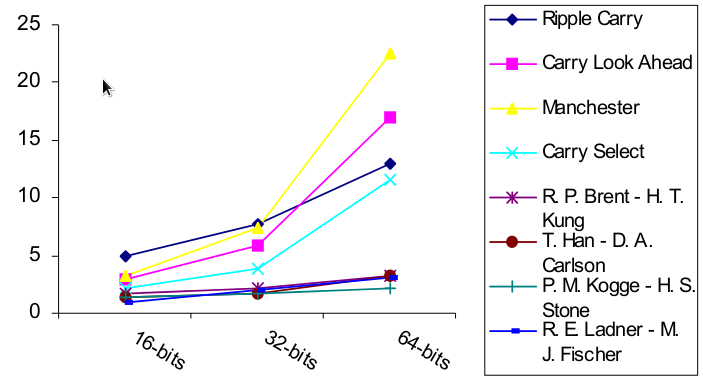
\includegraphics[scale=0.39]{figuras/retardo-bits.png}
  \caption{Retardo respecto al tama�o de los operandos}
  \label{retardo-bits}
\end{figure}


\end{frame}
\begin{frame}{Dise�o digital}
  Selecci�n de la arquitectura.

\begin{figure}[h]
  \centering
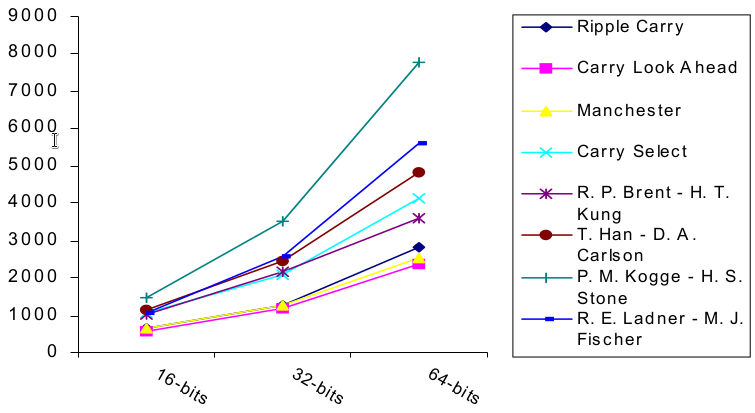
\includegraphics[scale=0.39]{figuras/area-bits.png}
\vspace{-1pt}
  \caption{�rea respecto al tama�o de los operandos}
  \label{area-bits}
\vspace{-15pt}
\end{figure}
\end{frame}

\begin{frame}{}
\begin{table}[h]
\centering
\begin{tabular}{|l|l|l|}
\hline
\multicolumn{1}{|c|}{\textbf{Arquitectura}} & \multicolumn{1}{c|}{\textbf{Retardo M�x.   }} & \multicolumn{1}{c|}{\textbf{�rea}} \\ \hline
Ripple Carry  & \(O(n)\) & \(O(n)\) \\ \hline
Carry Look-Ahead  & \(O(\log_2(n))\) & \(O(n\log_2(n))\) \\ \hline
Ladner-Fisher &\( O(\log_2(n))\) & \(O(n\log_2(n))   \) \\ \hline
Sklansky &\( O(\log_2(n))\) & \(O(n\log_2(n))\) \\ \hline
Kogge-Stone & \( O(\log_2(n))\) & \(O(n\log_2n)\)\\ \hline
%Han-Carlson & \( O(\log_2(n))\) &... \\ \hline % Lo quito ya que no encuentro la funci�n de complejidad de �rea.
Brent-Kung & $O(\log_2(n))$ & \(O(n)\) \\ \hline
\end{tabular}
\caption{Resumen de las funciones de retardo y �rea de algunos sumadores}\label{tabla:sumadores}
\end{table}
\hyperlink{sumadorPP}{\beamergotobutton{Implementaci�n}}
  \hypertarget{return}{}

\end{frame}
%----------------------------------------------------------------------------------
\begin{frame}{Carry Look-ahead}

Ya que una vez que el acarreo en la posici�n \(i\) es conocido, se puede calcular la suma como:
\begin{equation}\label{s_i}
s_i = a_i \oplus b_i\oplus c_i
\end{equation}

El acarreo se \emph{genera} � se \emph{propaga}, seg�n las siguientes ecuaciones:

%\vee es el OR
%\wedge es el AND
%\oplus es el XOR
%$$a_i=\lnot{a_i}\wedge\lnot{b_i}=\lnot{(a_i \vee b_i)}$$
$$g_i=a_ib_i$$
$$p_i=a_i \oplus b_i$$

C�lculo recursivo del acarreo:
\begin{equation}
%c_{i+1}=g_i\vee (c_i \wedge p_i)
c_{i+1}=g_i + c_i p_i
\end{equation}

\end{frame}
%----------------------------------------------------------------------------------
\begin{frame}{Desenrollando la recurrencia del acarreo}
Uno puede desenrollar esta f�rmula recursiva del acarreo hasta lograr una funci�n que dependa directamente de los operandos ($a$ y $b$) y del acarreo de entrada $c_{\text{in}}$:
\scriptsize{
\begin{equation}
\begin{aligned}
c_i &= g_{i-1} + p_{i-1}c_{i-1}\notag\\
&=g_{i-1}+p_{i-1}(g_{i-2}+p_{i-2}c_{i-2})=g_{i-1}+p_{i-1}g_{i-2}+p_{i-1}p_{i-2}c_{i-2}\notag\\
&=g_{i-1} + p_{i-1}g_{i-2}+p_{i-1}p_{i-2}g_{i-3}+p_{i-1}p_{i-2}p_{i-3}c_{i-3}\notag\\
&=g_{i-1} +p_{i-1}g_{i-2}+p_{i-1}p_{i-2}g_{i-3}+p_{i-1}p_{i-2}p_{i-3}g_{i-4}+p_{i-1}p_{i-2}p_{i-3}p_{i-4}c_{i-4}\label{gyp}	
\end{aligned}
\end{equation}
}
\end{frame}

%----------------------------------------------------------------------------------
\begin{frame}
Podemos interpretar estas ecuaciones de la siguiente forma: las cuatro posiciones de bits propagan colectivamente un acarreo $c_\text{in}$ si y solo s� cada una de las posiciones propaga; y el bloque gener	a un acarreo si en la posici�n $i+3$ se genera uno, o se podrouce en la posici�n $i+2$ y es propagado por la posici�n $i+3$, etc.
\end{frame}
%----------------------------------------------------------------------------------
\begin{frame}{Problema de prefijos paralelos}

\begin{equation}
\begin{aligned}
\text{Dado:}\\
 & \text{Entradas:} x_0,x_1,\dotsc,x_{k-1} \\
 & \text{Un operador + asociativo}\\ 
\text{Computar}:&x_0 \nonumber \\
&x_0+x_1 \nonumber \\ 
&x_0+x_1+x_2 \nonumber \\ 
&\vdots \nonumber \\ 
&x_0+x_1+x_2+\dotsb+x_{k-1} \nonumber
\end{aligned}
\end{equation}

\end{frame}


%----------------------------------------------------------------------------------
\begin{frame}{C�mputo del acarreo como un problema de prefijos paralelos}
 
Pensemos la ecuaci�n \ref{gyp} de la siguiente forma, asumiendo que $c_0=c_\text{in}$ viene desde otro bloque:
\begin{equation}
\begin{aligned}
g_{[i,i+3]} &= g_{i+3}+g_{i+2}p_{i+3}+g_{i+1}p_{i+2}p_{i+3}+g_{i}p_{i+1}p_{i+2}p_{i+3}\nonumber\\
p_{[i,i+3]} &= p_{i}p_{i+1}p_{i+2}p_{i+3}\nonumber
\end{aligned}
\end{equation}
\end{frame}
%----------------------------------------------------------------------------------

\begin{frame}{C�mputo del acarreo como un problema de prefijos paralelos}
  \scriptsize{
\begin{equation}\label{eq:ppProblem}
\begin{aligned}
\text{Dados:}\\
 & \text{Entradas:} (g_0,p_0),(g_1,p_1),\dotsc,(g_{k-1},p_{k-1}) \\
 & \text{Un operador} \circ \text{asociativo}\\ 
\text{Computar}:\\
(G_0,P_0) = &(g_{[0,0]},p_{[0,0]})\\
(G_1,P_1) = &(g_{[0,0]},p_{[0,0]})\circ(g_{[0,1]},p_{[0,1]})\\
&\vdots  \\
(G_{k-1},P_{k-1}) = &(g_{[0,0]},p_{[0,0]})\circ(g_{[0,1]},p_{[0,1]})\dotsc \circ(g_{[0,k-2]},p_{[0,k-2]})\circ(g_{[0,k-1]},p_{[0,k-1]}) \nonumber
\end{aligned}
\end{equation}
}
\end{frame}
%-------------------------------------------------------------------------
\begin{frame}{Operador de Brent-Kung}
El operador $\circ$ se define como:
\begin{equation}
(g,p) \circ (\hat{g},\hat{p}) = (g\vee(p\wedge\hat{g}),p\wedge\hat{g})\label{gap}
\end{equation}

\begin{figure}[h!]
  \centering
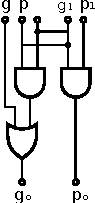
\includegraphics[scale=1.0]{figuras/dotOp_schem.pdf}
%\vspace{-5pt}
  \caption{Operator Punto de Brent-Kung}
  \label{dotOp}
%\vspace{-15pt}
\end{figure}
\end{frame}
%-------------------------------------------------------------------------

\begin{frame}[label=sumadorPP]
\begin{figure}[h]
  \centering
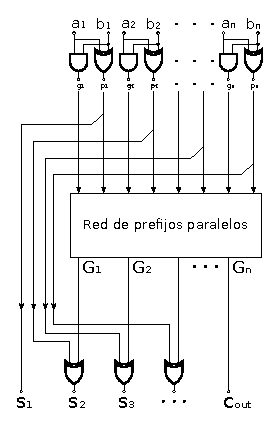
\includegraphics[scale=1.0]{figuras/arquitectura_schem_generico.eps}
  \caption{Sumador de prefijo paralelo}
  \label{fig:ppadder}
\end{figure}

\end{frame}
%----------------------------------------------------------------------------------
\begin{frame}

\begin{figure}[h!]
\vspace{-5pt}
  \centering
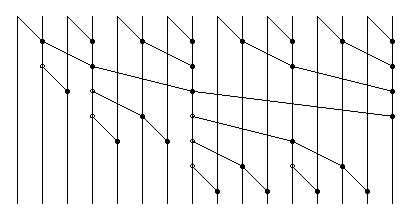
\includegraphics[scale=1.4]{figuras/bKung16.eps}
  \caption{Red de prefijo paralelo para Brent-Kung (ejemplo de 16 bits)}
\label{bKung16}
\vspace{-10pt}
\end{figure}

\end{frame}
%-------------------------------------------------------------------------
\begin{frame}
\begin{figure}[h]
  \centering
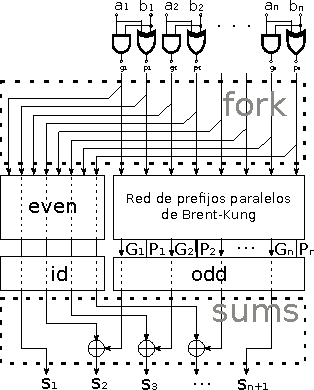
\includegraphics[scale=1.0]{figuras/arquitectura_schem.pdf}
  \caption{Sumador de Brent-Kung}
  \label{fig:bkungadder}
\end{figure}
\end{frame}
%-------------------------------------------------------------------------


\begin{frame}
\begin{figure}[h!]
\vspace{-5pt}
  \centering
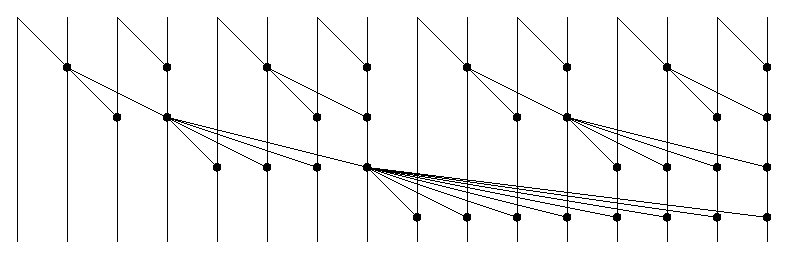
\includegraphics[scale=0.7]{figuras/sklansky16.eps}
  \caption{Red de prefijo paralelo para Sklansky (ejemplo de 16 bits)}
\label{fig:sklansky16}
\vspace{-10pt}
\end{figure}\end{frame}

%-------------------------------------------------------------------------
\begin{frame}{Implementaci�n de los circuitos en lenguaje de descripci�n de hardware}
\end{frame}
%-------------------------------------------------------------------------
\begin{frame}{Nuevos lenguajes de descripci�n de hardware}
 \begin{itemize}
    \item Usar un �nico lenguaje para describir, simular, verificar e implementar el circuito
    \item Los circuitos se describen en Haskell, Scala o Python, el HDL es simplemente un conjunto de m�dulos o librer�as
    \item Generar autom�ticamente una descripci�n en VHDL o Verilog
    \item Describir circuitos que construimos a partir de subcircuitos, adem�s de la posibilidad de reutilizar f�cilmente patrones de conexi�n
 \end{itemize}


\end{frame}
%-------------------------------------------------------------------------

\begin{frame}{�Por qu� Lava?}
  \begin{itemize}
    \item Conocimiento previo del lenguaje
    \item Genera un netlist VHDL (F�cil integraci�n con Electric)
    \item Los circuitos son descriptos como funciones que operan sobre listas, tuplas o sobre circuitos
    \item F�cil integraci�n con un SAT solver para verificaci�n formal
  \end{itemize}

\end{frame}
%-------------------------------------------------------------------------

\begin{frame}[fragile]{Operador de Brent-Kung en Lava}
A partir de la definici�n del operador:
\begin{equation*}
(g,p) \circ (\hat{g},\hat{p}) = (g\vee(p\wedge\hat{g}),p\wedge\hat{g})\label{gap}
\end{equation*}
En Lava la escribimos:

\lstset{language=Haskell}
\begin{lstlisting}
dotOp ((g1, p1) ,(g, p)) = (go, po)
   where
      go = or2 (g, and2 (p, g1))
      po = and2 (p, p1)
\end{lstlisting}
\end{frame}
%-------------------------------------------------------------------------
\begin{frame}[fragile]{Red de prefijo paralelo de Brent-Kung en Lava}
Funciones auxiliares:
  \begin{figure}
    \centering
    
\includegraphics[scale=2.00]{figuras/wrapR.eps}
 \end{figure}
\end{frame}
%-------------------------------------------------------------------------
\begin{frame}[fragile]
  \begin{lstlisting}
comb []     = []
comb [a]    = []
comb (a:as) = dop [a, head as] ++ comb (tail as)
--
posComb (a:as)  = a: (comb (init as))++ [last as]
--
half p = unzipl ->- (id -|- p) ->- zipl
--
wrap p = comb ->- half p ->- posComb 
\end{lstlisting}
\end{frame}
%-------------------------------------------------------------------------
\begin{frame}[fragile]
\noindent Luego finalemente, podemos describir {\verb|ppNet|}:

 \begin{figure}
    \centering
    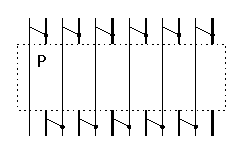
\includegraphics[scale=2.0]{figuras/sheeranrecurrence.eps}
 \end{figure}

\begin{lstlisting}
ppNet [a]    = []
ppNet [a, b] = dop [a, b]
ppNet as     = wrap ppNet as
\end{lstlisting}

\end{frame}
%-------------------------------------------------------------------------






%\begin{frame}{Automatic optimal pp-partitioning is hopeless, but\dots}
%  \begin{itemize}
%  \item The hardness results are \alert{worst-case} results for\\
%    \alert{highly artificial inputs}.
%  \item \alert{Real biological data} might have special properties
%    that make the problem \alert{tractable}.
%  \item One such property is that perfect phylogenies are often
%    perfect \alert{path} phylogenies:
%
%    In HapMap data, in 70\% of the blocks where a perfect phylogeny
%    is possible a perfect path phylogeny is also possible.
%  \end{itemize}  
%\end{frame}
%
%
%\begin{frame}{Example of a perfect path phylogeny.}
%  \begin{columns}[t]
%    \column{.3\textwidth}
%    \begin{exampleblock}{Genotype matrix}
%      $G\colon$
%      \begin{tabular}{ccc}
%        A & B & C \\\hline
%        2 & 2 & 2 \\
%        0 & 2 & 0 \\
%        2 & 0 & 0 \\
%        0 & 2 & 2 
%      \end{tabular}
%    \end{exampleblock}
%
%    \column{.3\textwidth}
%    \begin{exampleblock}{Haplotype matrix}
%      $H\colon$
%      \begin{tabular}{ccc}
%        A & B & C \\\hline
%        1 & 0 & 0 \\
%        0 & 1 & 1 \\
%        0 & 0 & 0 \\
%        0 & 1 & 0 \\
%        0 & 0 & 0 \\
%        1 & 0 & 0 \\
%        0 & 0 & 0 \\
%        0 & 1 & 1 
%      \end{tabular}
%    \end{exampleblock}
%
%    \column{.4\textwidth}
%    \begin{exampleblock}{Perfect path phylogeny}
%      \begin{center}
%        \begin{tikzpicture}[auto,thick]
%          \tikzstyle{node}=%
%          [%
%            minimum size=10pt,%
%            inner sep=0pt,%
%            outer sep=0pt,%
%            ball color=example text.fg,%
%            circle%
%          ]
%        
%          \node [node] {} [->]
%            child {node [node] {} edge from parent node[swap]{A}}
%            child {node [node] {}
%              child {node [node] {} edge from parent node{C}}
%              edge from parent node{B}
%            };
%        \end{tikzpicture}
%      \end{center}
%    \end{exampleblock}
%  \end{columns}
%\end{frame}
%
%
%\begin{frame}{The modified formal computational problem.}
%  We are interested in the computational complexity of \\
%  the function $\chi_{\alert{\operatorname{PPP}}}$:
%  \begin{itemize}
%  \item It gets genotype matrices as input.
%  \item It maps them to a number $k$.
%  \item This number is minimal such that the sites can be
%    covered by $k$ sets, each admitting a perfect \alert{path} phylogeny.
%    \\
%    (We call this a ppp-partition.)
%  \end{itemize}
%\end{frame}
%-------------------------------------------------------------
\subsection{Dise�o f�sico}
\begin{frame}{Flujo de dise�o f�sico}
\begin{figure}[h]
\centering
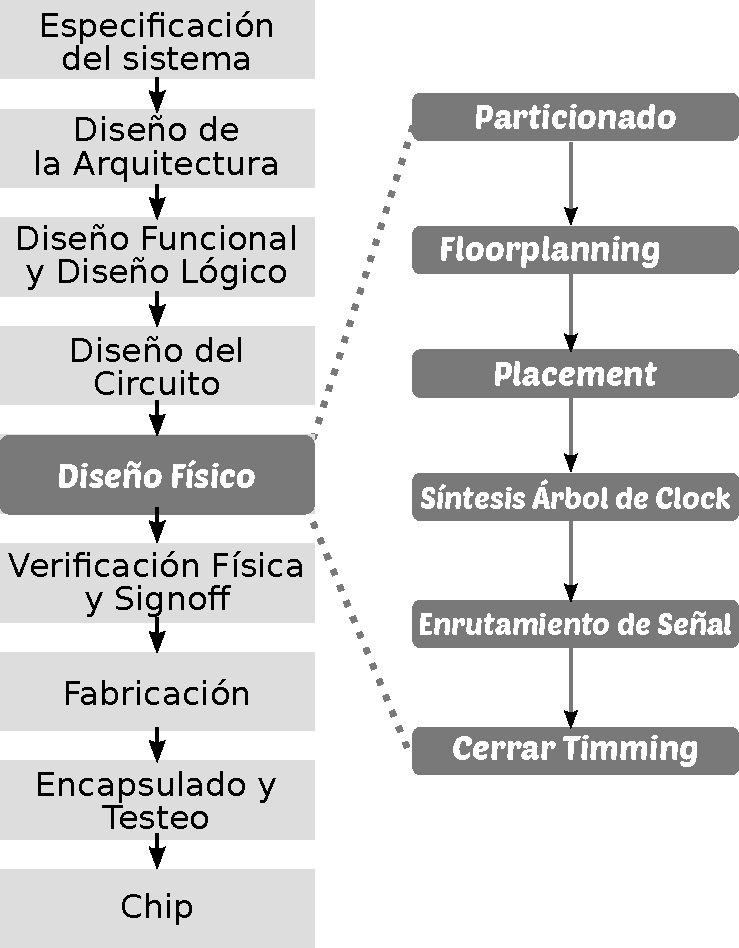
\includegraphics[scale=0.43]{figuras/DisenioFisico.pdf}
  \label{fig:dise�oF�sico}
\end{figure}
\end{frame}
%------------------------------------------------------------
\begin{frame}{Selecci�n del proceso de fabicaci�n}
  Seleccionamos TSMC 180nm por las siguientes razones:
  \begin{itemize}
      \item Existen herramientas de software libre para esta tecnolog�a.
      \item Bajo costo de fabricaci�n 
      \item Posibilidad de integrar sistemas de gran complejidad y alta performance
    \end{itemize}

\end{frame}
%-------------------------------------------------------------
\begin{frame}{Selecci�n del proceso de fabicaci�n}
Ejemplos de microprocesadores que fueron fabricados en esta tecnolog�a:

\begin{table}[h]
\centering
\begin{tabular}{@{}lc@{}}
\toprule
Procesador             & A�o de lanzamiento \\ \midrule
Intel Coppermine E                & 1999             \\
AMD Athlon Thunderbird      & 2000             \\
Intel Celeron (Willamette)               & 2002            \\
Motorola PowerPC 7445 y 7455 (Apollo 6) & 2002           \\ \bottomrule
\end{tabular}
\caption{Procesadores fabricados en CMOS 180nm }
\label{tab:procesadores180nm}
\end{table}
\end{frame}
%-------------------------------------------------------------
\begin{frame}{}
\end{frame}
%-------------------------------------------------------------
\begin{frame}{Reglas de dise�o para TSMC 180nm}
  MOSIS denomina a las reglas de dise�o \textbf{SCN6M\_DEEP}, que significa:
%El proceso nos ofrece 6 capas de metal (aluminio) para la interconexi�n, 1 capa de silicio policristalino (\emph{poly}) para crear la compuerta y tambi�n para la interconexi�n de las mismas (distancias cortas s�lamente, por su mayor resistividad que el cobre), con 2 tipos de �xidos para crear el aislante de las compuertas, los que pueden ser alimentados con tensi�n m�xima de 1,8V, y los que pueden ser alimentados con 3,3V (pensados principalmente como transistores para los circuitos de entrada y salida del chip). MOSIS denomina a las reglas de dise�o que utilizaremos para esta tecnolog�a como SCN6M\_DEEP, que significa:\begin{frame}{180nm TSMC}
  \begin{itemize}
    \item S: Escalable
    \item C: Tecnolog�a de fabricaci�n CMOS
    \item N: Pozo N.
    \item 6M: 6 metales y un conductor policristalino (\emph{poly}) para crear las compuertas.
    \item DEEP: Reglas \emph{deep submicron} (lamda 90nm).
  \end{itemize}
\end{frame}
%-------------------------------------------------------------
\begin{frame}{Mapeo de l�gica a compuertas}
Mapeo de una funci�n l�gica a una celda est�ndar
\begin{figure}[h]
\centering
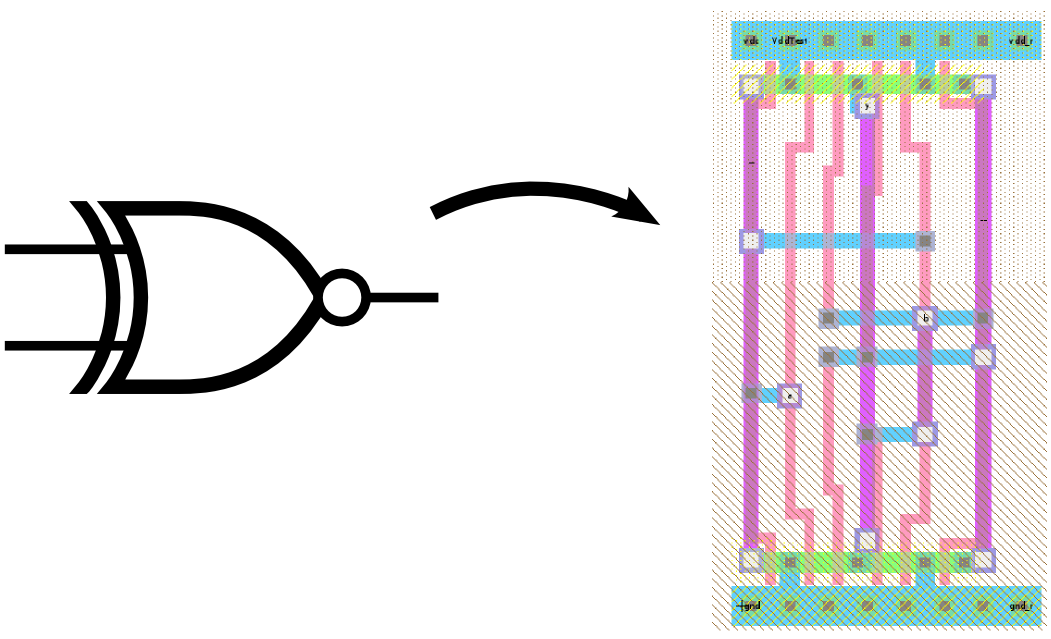
\includegraphics[scale=0.59]{figuras/map-xnor.png}
  \label{fig:map-xnor}
\end{figure}
\end{frame}
%------------------------------------------------------------
\begin{frame}{Librer�a de celdas est�ndar}
\begin{figure}
        \centering
        \begin{subfigure}[b]{0.20\textwidth}
                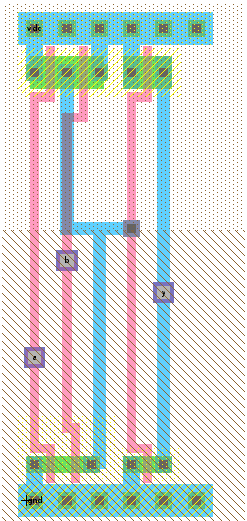
\includegraphics[width=1.075\textwidth]{figuras/and2_1x.png}
                \caption{and2}
                \label{fig:gull}
        \end{subfigure}\quad
        \begin{subfigure}[b]{0.20\textwidth}
                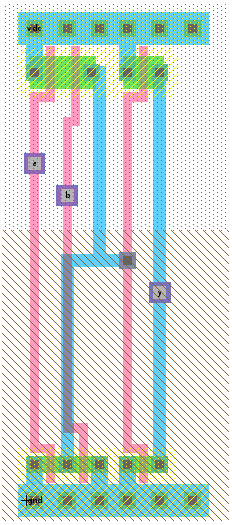
\includegraphics[width=1\textwidth]{figuras/or2_1x.png}
                \caption{or2}
                \label{fig:tiger}
        \end{subfigure} 
        \begin{subfigure}[b]{0.20\textwidth}
                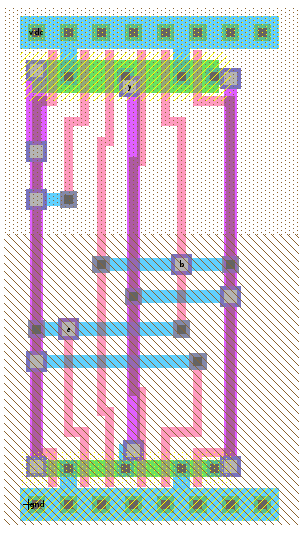
\includegraphics[width=1.31\textwidth]{figuras/xor2_1x.png}
                \caption{xor}
                \label{fig:mouse}
        \end{subfigure}\qquad
        \begin{subfigure}[b]{0.20\textwidth}
                \includegraphics[width=0.845\textwidth]{figuras/id_1x_.png}
                \caption{buffer}
                \label{fig:mouse}
        \end{subfigure}
        \caption{Conjunto de celdas est�ndar}\label{fig:animals}
\end{figure}
\end{frame}

%------------------------------------------------------------

\begin{frame}{Celdas est�ndar}
Grilla de interconexionado y riel de alimentaci�n de las celdas est�ndar de $128 \lambda$
 \begin{figure}[h]
\centering
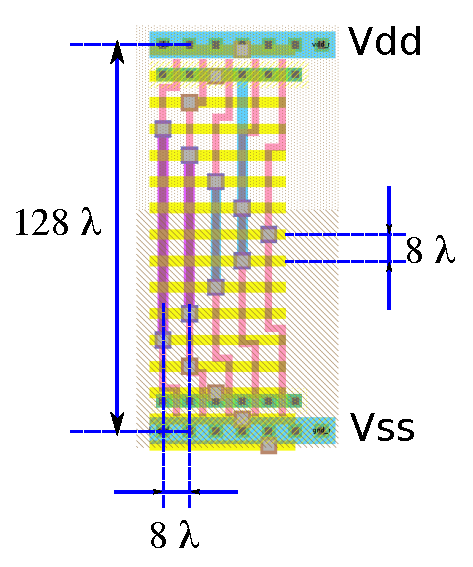
\includegraphics[scale=.7]{figuras/CeldEstandarAlto.eps}
  \label{fig:pitchCeldaEstandar}
\end{figure}
\end{frame}
%------------------------------------------------------------



\begin{frame}{Ubicaci�n y conexionado del \textit{ripple carry adder}}
\begin{table}[h]
\centering
\resizebox{\textwidth}{!}{%
\begin{tabular}{@{}cccc|ccc|ccc@{}}
\toprule
\multicolumn{1}{l}{\textbf{Ripple Carry}} & \multicolumn{3}{c}{8 bits}    & \multicolumn{3}{c}{16 bits}      & \multicolumn{3}{c}{32 bits}      \\ \midrule
filas                                     & 3      & \alert{4}      & 5      & 5       & \alert{6}       & 7       & \alert{8}       & 7       & 6       \\
ancho                                     & 1297   & 966    & 843    & 1562    & 1350    & 1142    & 1881    & 2169    & 2581    \\
alto                                      & 665    & 839    & 958    & 1227    & 1196    & 1600    & 2000    & 1850    & 1360    \\
�rea                                      & 862505 & 810474 & 807594 & 1916574 & 1614600 & 1827200 & 3762000 & 4012650 & 3510160 \\
ancho/alto                                & 0,51   & 0,87   & 1,14   & 0,79    & 0,89    & 1,40    & 1,06    & 0,85    & 0,53    \\ \bottomrule
\end{tabular}
}
\caption{Las dimensiones de los lados y el �rea est�n en $\lambda$ y $\lambda^2$ respectivamente.}
\label{tab:rippleCarry}
\end{table}

\end{frame}
%------------------------------------------------------------
\begin{frame}{Ubicaci�n y conexionado del sumador de \textit{Brent-Kung}}
\begin{table}[h]
\centering
\resizebox{\textwidth}{!}{%
\begin{tabular}{@{}cccc|cccc|cccc@{}}
\toprule
\textbf{Brent-Kung} & \multicolumn{3}{c}{8 bits}      & \multicolumn{4}{c}{16 bits}                & \multicolumn{4}{c}{32 bits}                \\ \midrule
filas               & 3       & \alert{4}     & 5       & 4       & 5       & \alert{6}       & 7       & 6       & \alert{7}       & 8       & 9       \\
ancho               & 1386    & 1090   & 945     & 2268    & 1757    & 1545    & 1429    & 3196    & 1983    & 2569    & 2424    \\
alto                & 746     & 910    & 1199    & 1255    & 1436    & 1540    & 1959    & 2024    & 2871    & 2927    & 2882    \\
�rea                & 1033956 & 991900 & 1133055 & 2846340 & 2523052 & 2379300 & 2799411 & 6468704 & 5693193 & 7519463 & 6985968 \\
ancho/alto          & 0,54    & 0,83   & 1,27    & 0,55    & 0,82    & 1,00    & 1,37    & 0,63    & 1,45    & 1,14    & 1,19    \\ \bottomrule
\end{tabular}
}
\caption{Las dimensiones de los lados y el �rea est�n en $\lambda$ y $\lambda^2$ respectivamente.}

\label{tab:brent-kung}
\end{table}


\end{frame}
%------------------------------------------------------------
\begin{frame}{Ubicaci�n y conexionado del sumador de \textit{Sklansky}}
\begin{table}[h]
\centering
\resizebox{\textwidth}{!}{%
\begin{tabular}{@{}cccc|cccc|ccc@{}}
\toprule
\textbf{Sklansky} & \multicolumn{3}{c}{8 bits}       & \multicolumn{4}{c}{16 bits}                & \multicolumn{3}{c}{32 bits}      \\ \midrule
filas              & 3       & \alert{4}       & 5       & 4       & \alert{5}       & 6       & 7       & 6       & \alert{7}       & 8       \\
ancho              & 1516    & 1167    & 954     & 3538    & 2042    & 1825    & 1536    & 3678    & 3229    & 2860    \\
alto               & 810     & 973     & 1252    & 1345    & 1581    & 1878    & 2063    & 2639    & 2695    & 3072    \\
�rea               & 1227960 & 1135491 & 1194408 & 4758610 & 3228402 & 3427350 & 3168768 & 9706242 & 8702155 & 8785920 \\
ancho/alto         & 0,53    & 0,83    & 1,31    & 0,38    & 0,77    & 1,03    & 1,34    & 0,72    & 0,83    & 1,07    \\ \bottomrule
\end{tabular}
}
\caption{Las dimensiones de los lados y el �rea est�n en $\lambda$ y $\lambda^2$ respectivamente.}
\label{tab:sklansky}
\end{table}
\end{frame}
%------------------------------------------------------------
\begin{frame}{\textit{Layout} de todas las arquitecturas y tama�os}
  \begin{figure}
  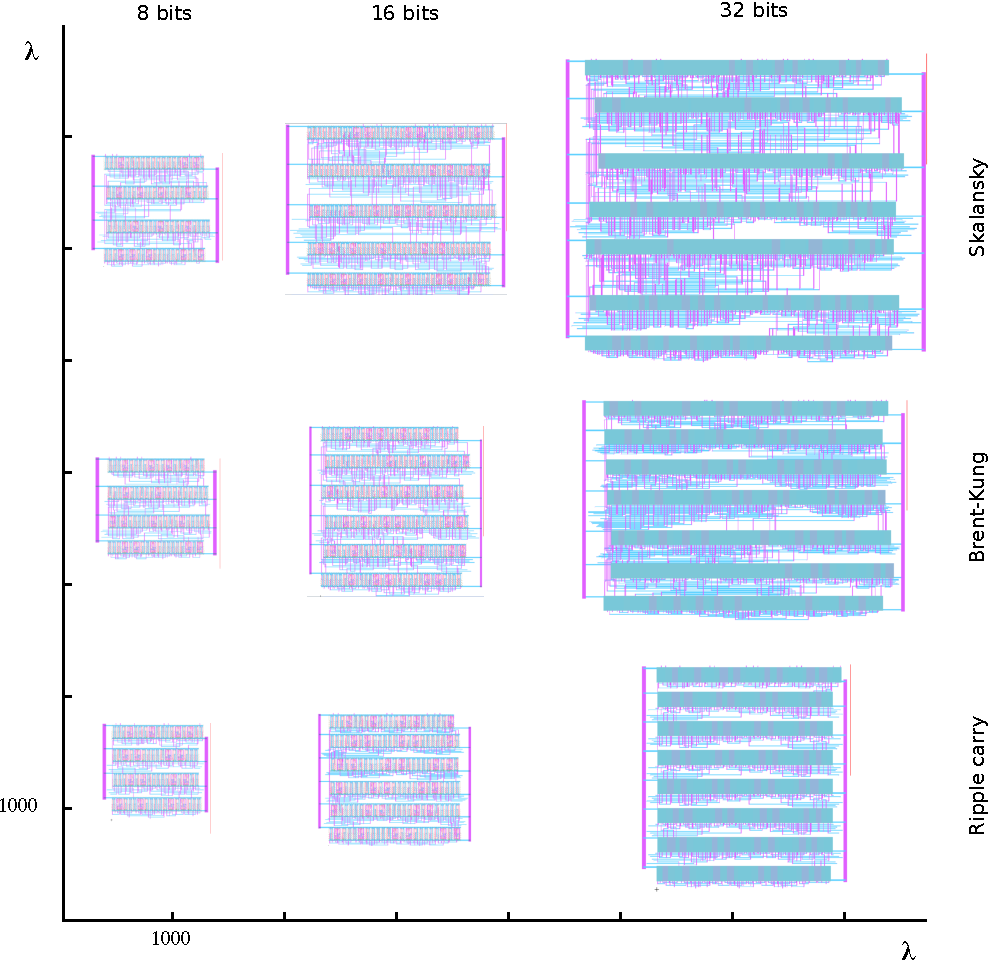
\includegraphics[scale=0.450]{figuras/layout-disenos.pdf}
  \end{figure}
\end{frame}
%-------------------------------------------------------------

\begin{frame}{Simulaci�n post \emph{layout} para calcular performance y potencia}
Realizamos extracci�n de par�sitos del \cursi{layout} y utililizamos un motor de simulaci�n anal�gico tipo SPICE, llamado gnucap.
\end{frame}
%-------------------------------------------------------------
\begin{frame}{Flujo para simulaciones anal�gicas}
 \begin{figure}[h]
  \centering
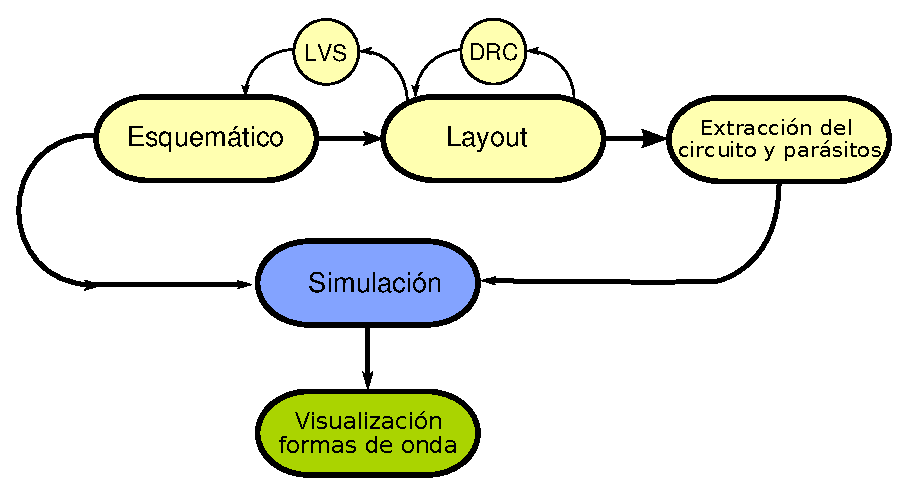
\includegraphics[scale=0.68]{figuras/analog-flow.eps}
\label{fig:aflow}
%\vspace{-10pt}
\end{figure}
\end{frame}
%%-------------------------------------------------------------
\begin{frame}{Retardo de propagaci�n}
  \alert{Definici�n:}

Retardo de propagaci�n de un inversor:
\begin{figure}[h]
\centering
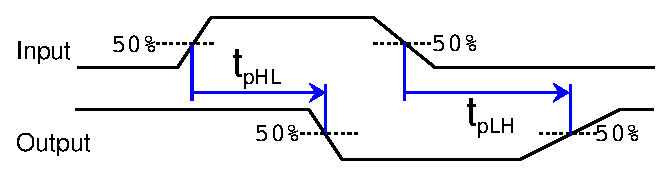
\includegraphics[scale=0.65]{figuras/tiempo_retardo_tpHL-tpLH.eps}
  \label{fig:propagationDelay}
\end{figure}

Se define usualmente el retardo de propagaci�n como:

$$ t_p = \frac{t_{pLH} + t_{pHL}}{2} $$

\end{frame}
%-------------------------------------------------------------
\begin{frame}{Simulaci�n post \emph{layout} para calcular performance}
\begin{figure}
  \centering
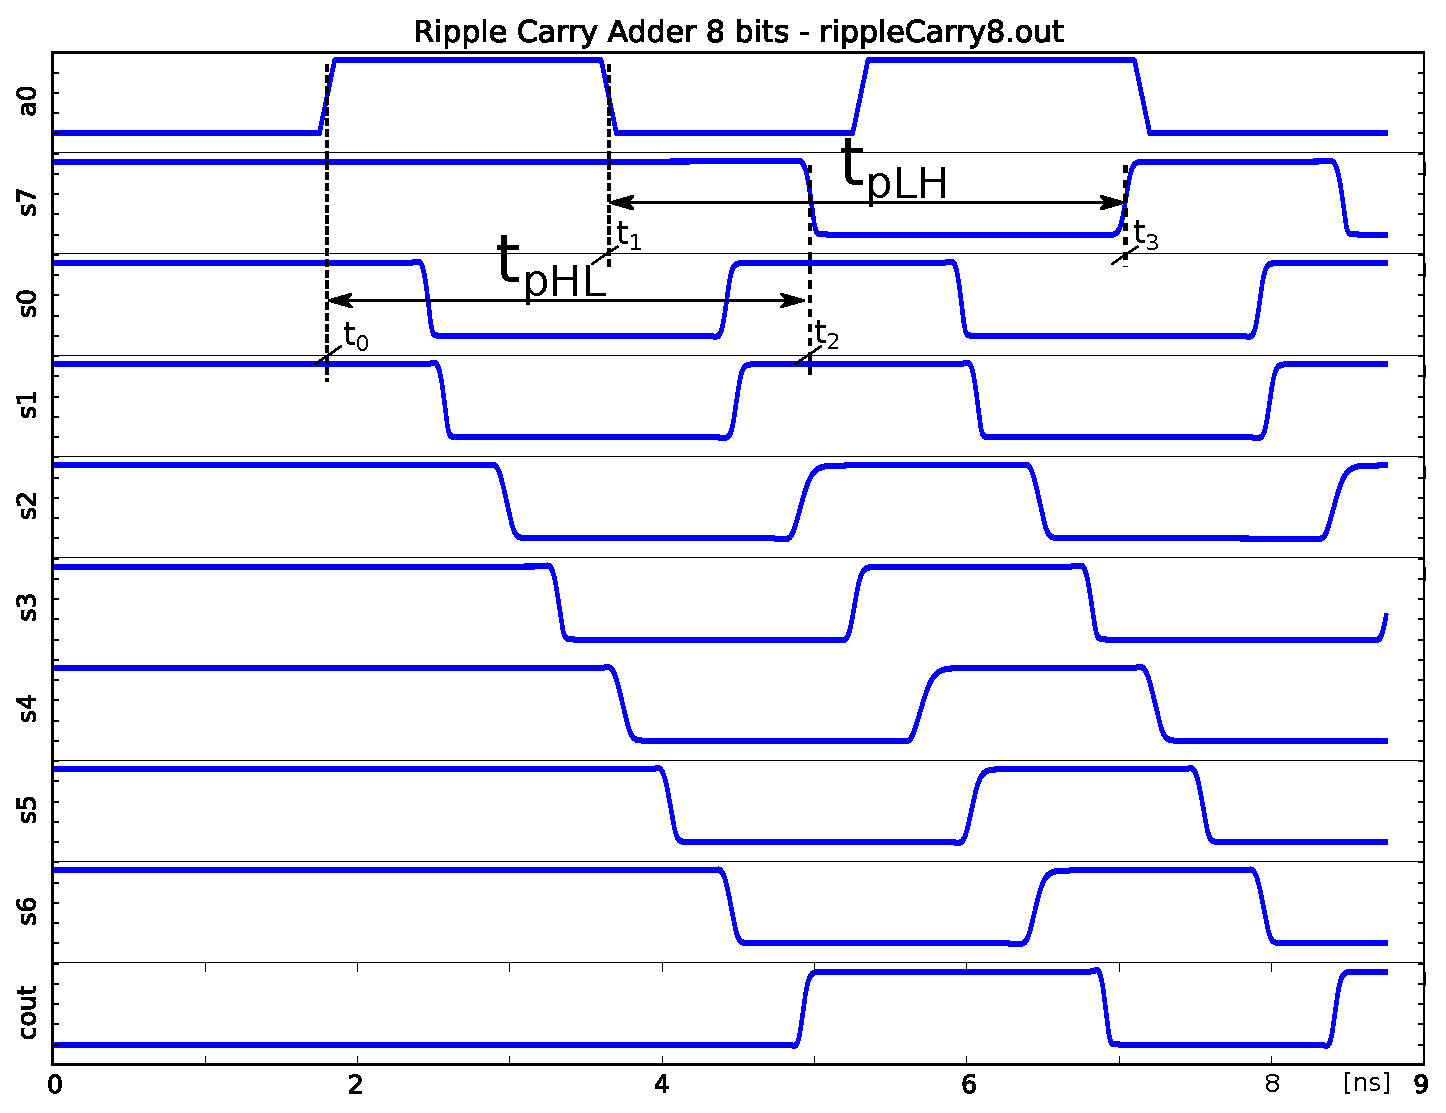
\includegraphics[scale=.36]{figuras/sim_rca8bits_.eps}
\end{figure}
\end{frame}
%-------------------------------------------------------------
\begin{frame}{Simulaci�n post \emph{layout} para calcular performance }
Sumador de 8 bits de \cursi{ripple carry}
\begin{figure}
  \centering
 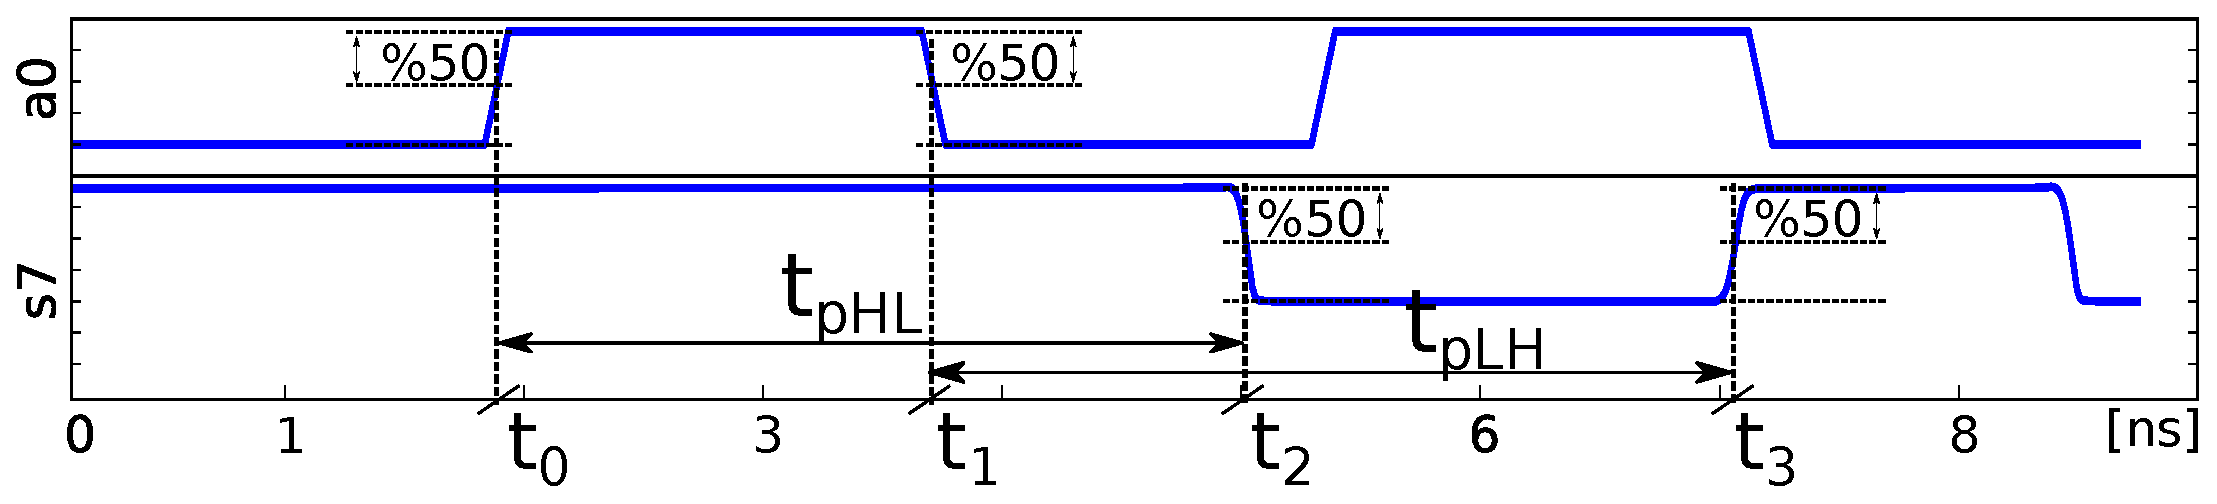
\includegraphics[scale=.29]{figuras/rca8bits_zoom.eps}
\end{figure}

$$t_{pHL} = t_2 - t_0 = 5.01~\ns - 1.8~\ns = 3.21~\ns$$
$$t_{pLH} = t_3 - t_1 = 7.05~\ns - 3.61~\ns = 3.44~\ns$$
$$t_p = \frac{(t_{pHL} + t_{pLH} )}{2} = 3.325~\ns$$
\end{frame}

%-------------------------------------------------------------
\begin{frame}{Potencia promedio disipada}
  \alert{Definici�n:}

La potencia promedio disipada total la podemos calcular si conocemos la corriente instant�nea que brinda la fuente de tensi�n $V_{DD}$, como podemos ver en la ecuaci�n \ref{eq:pv}.
\begin{figure}[h]
\centering
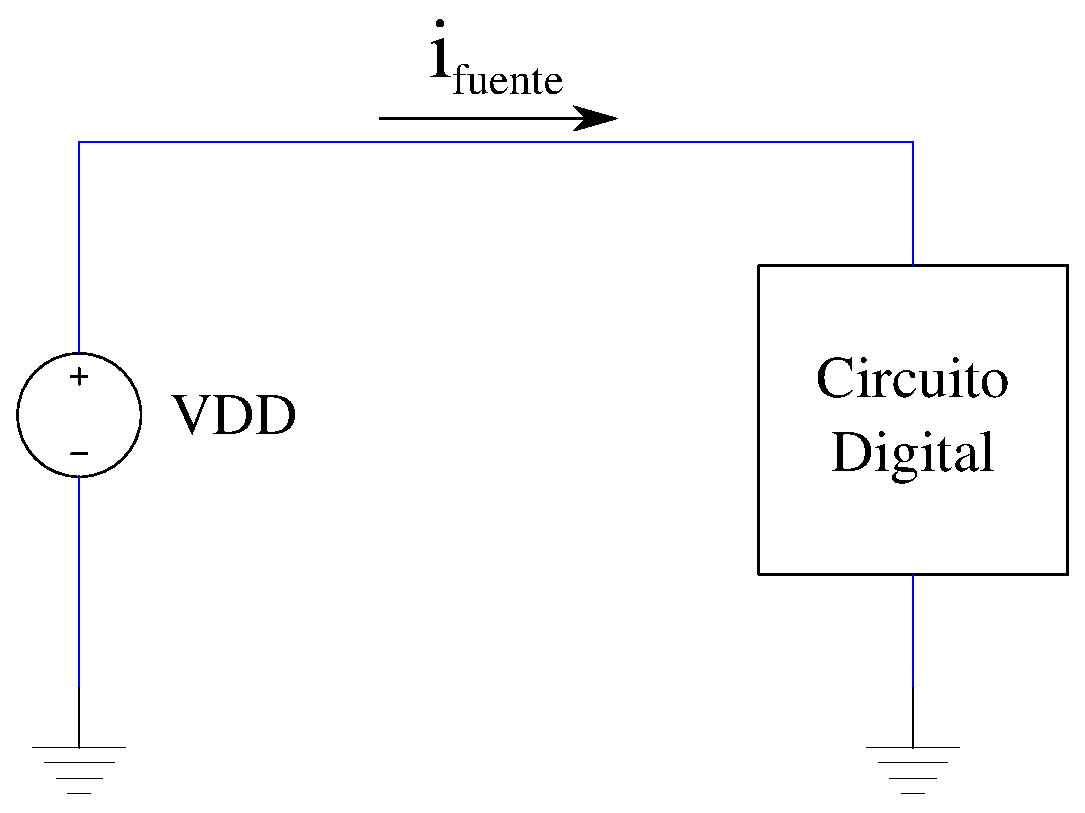
\includegraphics[scale=.21]{figuras/powerSupply.eps}
\end{figure}

\begin{equation}
P_{av} = \frac{1}{\mathrm{T}}\int\limits_0^T p(t)dt = \mathrm{\frac{V_{DD}}{T}}\int\limits_0^T i_{\mathrm{fuente}}(t)\mathrm{d}t 
\label{eq:pv}
\end{equation}
\end{frame}

%-------------------------------------------------------------
\begin{frame}{Simulaci�n de r�gimen transitorio del circuito Ripple Carry 8 bits}
\begin{figure}
  \centering
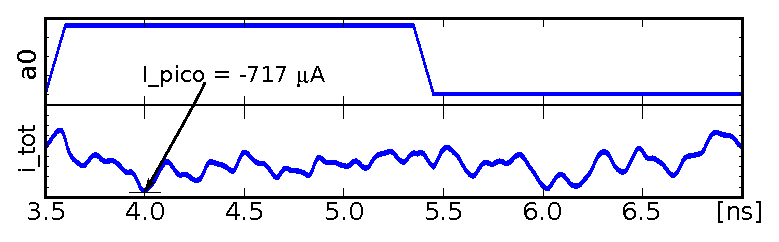
\includegraphics[scale=0.7]{figuras/rca8bits_power.eps}
\end{figure}
El per�odo de integraci�n que elegimos est� determinado por el $t_p$ del circuito, lo que f�sicamente quiere decir: Medimos la potencia del circuito cuando est� funcionando a la mayor velocidad posible. 
\end{frame}

\begin{frame}{Simulaci�n post \emph{layout} para calcular performance y potencia}
  \begin{block}{Simulaci�n post \cursi{layout}}
Realizamos las simulaciones de todas las arquitecturas y de los tres tama�os.
\end{block}
\end{frame}
%

%-------------------------------------------------------------
\begin{frame}{Resultados: Performance}
  \begin{figure}
  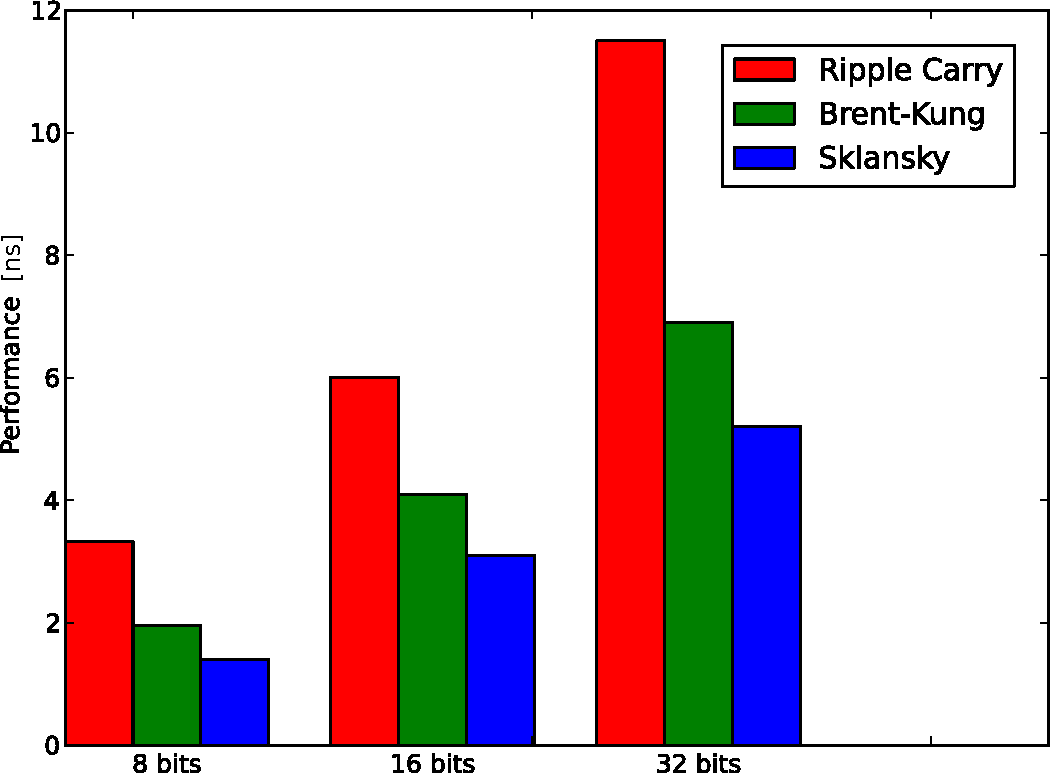
\includegraphics[scale=0.50]{figuras/barra_performance.pdf}
  \end{figure}
  \end{frame}
%-------------------------------------------------------------
\begin{frame}{Resultados: Potencia}
  \begin{figure}
  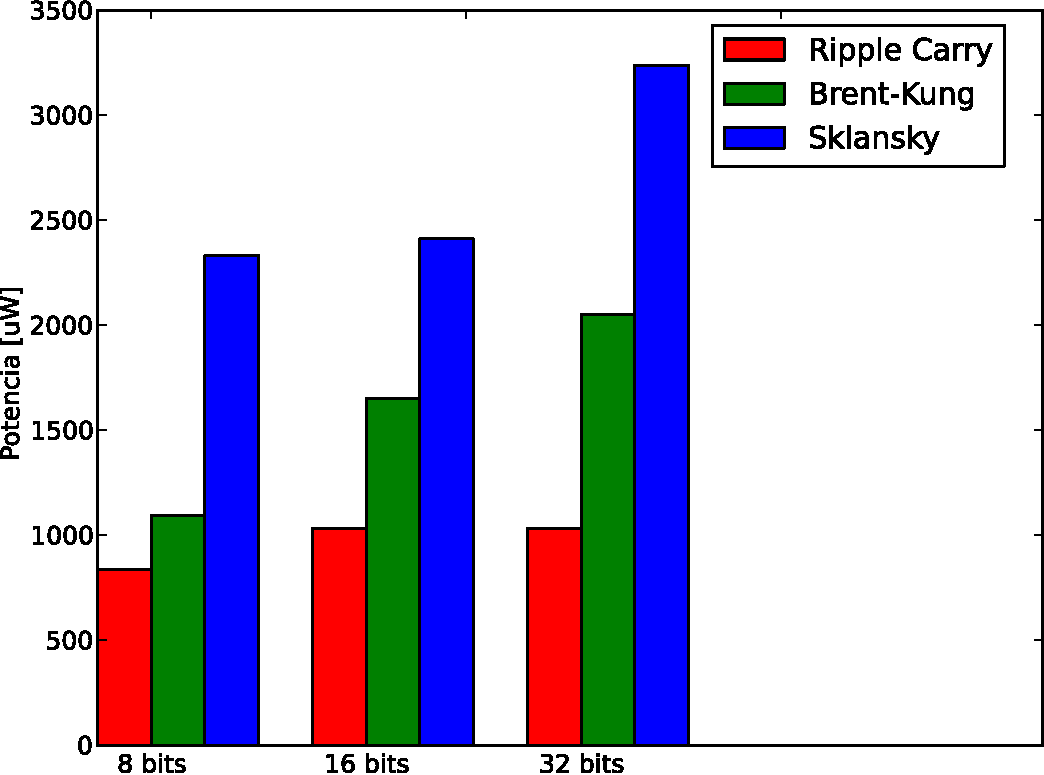
\includegraphics[scale=0.50]{figuras/barra_potencia2.pdf}
  \end{figure}
  \end{frame}
%-------------------------------------------------------------
\begin{frame}{Resumen}
Por lo tanto, hemos logrado un conjunto de sumadores que seg�n los requerimientos de �rea, potencia y performance, podremos elegir la arquitectura m�s adecuada. 

Para todos los tama�os de sumadores,   \begin{block}{Para sumadores de 32 bits}
La mayor velocidad se logra con Sklansky y el mejor compromiso entre velocidad, potencia y �rea con Brent-Kung. 
  \end{block}
  \begin{block}{Para todos los tama�os}
Si la performance no es un problema, un ripple carry es la soluci�n optima de estos tres, ya que ahorra �rea y energ�a.

  \end{block}


  \end{frame}
%-------------------------------------------------------------




%\begin{frame}{Good news about ppp-partitions of genotype matrices.}
%  \begin{theorem}
%    \alert{Optimal ppp-partitions of genotype matrices} can be
%    computed in \alert{polynomial time}. 
%  \end{theorem}
%  \begin{block}{Algorithm}
%    \begin{enumerate}
%    \item Build the following partial order:
%      \begin{itemize}
%      \item Can one column be above the other in a phylogeny?
%      \item Can the columns be the two children of the root of a
%        perfect path phylogeny?
%      \end{itemize}
%    \item Cover the partial order with as few compatible chain pairs 
%      as possible. 
%
%      For this, a maximal matching in a special graph needs to be
%      computed.
%    \end{enumerate}
%  \end{block}
%  \hyperlink{algorithm<1>}{\beamergotobutton{The algorithm in action}}
%  \hypertarget{return}{}
%\end{frame}

\section{Conclusiones}
\begin{frame}
  \frametitle<presentation>{Conclusiones}

  \begin{itemize}
  \item
    Sumadores r�pidos, eficientes o de bajo consumo.
  \end{itemize}
\end{frame}

%\begin{frame}
%  \frametitle<presentation>{Summary}
%
%  \begin{itemize}
%  \item
%    Finding optimal pp-partitions is \alert{intractable}. 
%  \item
%    It is even intractable to find a pp-partition when \alert{just two 
%      noncontiguous  blocks are known to suffice}.
%  \item
%    For perfect \alert{path} phylogenies, optimal partitions can be
%    computed \alert{in polynomial time}.
%  \end{itemize}
%\end{frame}
%

\appendix
\section{Resumen}
\begin{frame}{Resumen}
\end{frame}

%\begin{frame}[label=algorithm]{The algorithm in action.}{Computation of
%    the partial order.}
%  \begin{columns}[t]
%    \column{.4\textwidth}
%    \begin{exampleblock}{Genotype matrix}
%      $G\colon$
%      \begin{tabular}{ccccc}
%        A & B & C & D & E \\\hline
%        2 & 2 & 2 & 2 & 2 \\
%        0 & 1 & 2 & 1 & 0 \\
%        1 & 0 & 0 & 1 & 2 \\
%        0 & 2 & 2 & 0 & 0
%      \end{tabular}
%    \end{exampleblock}
%    \column{.6\textwidth}
%    \begin{exampleblock}{Partial order}
%      \begin{tikzpicture}[node distance=15mm]
%        \tikzstyle{every node}=
%        [%
%          fill=green!50!black!20,%
%          draw=green!50!black,%
%          minimum size=7mm,%
%          circle,%
%          thick%
%        ]
%
%        \node (A) {A};
%        \node (B) [right of=A] {B};
%        \node (C) [below of=B] {C};
%        \node (D) [above of=A] {D};
%        \node (E) [below of=A] {E};
%
%        \path [thick,shorten >=1pt,-stealth'] (A) edge (E)
%                         (B) edge (C)
%                         (D) edge (A)
%                             edge[bend right] (E);
%
%        \uncover<2>{
%        \path [-,blue,thick](A) edge (B)
%                                edge (C)  
%                            (B) edge (E)
%                            (C) edge (E);}
%      \end{tikzpicture}
%
%      Partial order: \tikz[baseline] \draw[thick,-stealth'] (0pt,.5ex)
%      -- (5mm,.5ex); 
%
%      \uncover<2>{\textcolor{blue}{Compatible as children of root:
%          \tikz[baseline] \draw[thick] (0pt,.5ex) -- (5mm,.5ex);}} 
%    \end{exampleblock}
%  \end{columns}  
%\end{frame}
%
%\begin{frame}{The algorithm in action.}{The matching in the special graph.}
%  \begin{columns}[t]
%    \column{.3\textwidth}
%    \begin{exampleblock}{Partial order}
%      \begin{tikzpicture}[node distance=15mm]
%        \tikzstyle{every node}=%
%        [%
%          fill=green!50!black!20,%
%          draw=green!50!black,%
%          minimum size=8mm,%
%          circle,%
%          thick%
%        ]
%
%        \node (A)              {$A$};
%        \node (B) [right of=A] {$B$};
%        \node (C) [below of=B] {$C$};
%        \node (D) [above of=A] {$D$};
%        \node (E) [below of=A] {$E$};
%
%        \path [thick,shorten >=1pt,-stealth'] (A) edge (E)
%                         (B) edge (C)
%                         (D) edge (A)
%                             edge[bend right] (E);
%
%        \path [-,blue,thick](A) edge (B)
%                                edge (C)  
%                            (B) edge (E)
%                            (C) edge (E);
%
%        \only<3->
%        {
%          \path[very thick,shorten >=1pt,-stealth',red] (D) edge (A) (B) edge (C);
%          \path [-,red,very thick](E) edge (B);
%        }
%      \end{tikzpicture}
%    \end{exampleblock}
%    \column{.7\textwidth}
%    \begin{exampleblock}{Matching graph}
%      \begin{tikzpicture}[node distance=15mm]
%        \tikzstyle{every node}=%
%        [%
%          fill=green!50!black!20,%
%          draw=green!50!black,%
%          minimum size=8mm,%
%          circle,%
%          thick,%
%          inner sep=0pt%
%        ]
%
%        \node (A)              {$A$};
%        \node (B) [right of=A] {$B$};
%        \node (C) [below of=B] {$C$};
%        \node (D) [above of=A] {$D$};
%        \node (E) [below of=A] {$E$};
%
%        \begin{scope}[xshift=4.75cm]
%          \node (A')               {$A'$};
%          \node (B') [right of=A'] {$B'$};
%          \node (C') [below of=B'] {$C'$};
%          \node (D') [above of=A'] {$D'$};
%          \node (E') [below of=A'] {$E'$};
%        \end{scope}
%        
%        \path [thick]    (A) edge (E')
%                         (B) edge (C')
%                         (D) edge (A')
%                             edge (E');
%
%        \path [blue,thick](A') edge (B')
%                               edge (C')  
%                          (B') edge (E')
%                          (C') edge (E');
%
%        \only<2->
%        {
%          \path[very thick,red] (D) edge (A')
%                           (B) edge (C')
%                           (B') edge (E');
%        }
%      \end{tikzpicture}
%    \end{exampleblock}
%  \end{columns}
%
%  \medskip
%  \uncover<2->{A \alert{maximal matching} in the matching graph
%    \uncover<3>{induces\\ \alert{perfect path phylogenies}.}}
%
%  \hfill\hyperlink{return}{\beamerreturnbutton{Return}}
%\end{frame}

\end{document}



\pagenumbering{Roman}

%\tableofcontents			%%% INCLUYE INDICE AL PRINCIPIO

\mainmatter
\hyphenation{ ba-yo-ne-ta re-vo-lu-cio-na-ria e-qui-va-le cul-tu-ral so-cia-lis-mo de-ma-sia-do ca-pi-ta-lis-tas in-ter-me-dios fun-cio-na-rios i-rrum-pir gue-rri-lla cons-tru-cción dia-rio re-vo-lu-ción en-tu-sias-mo te-ne-mos ra-di-cal-men-te nor-te-a-me-ri-ca-nos co-lo-ni-za-ción e-qui-va-le cul-tu-ral so-cia-lis-mo de-ma-sia-do ca-pi-ta-lis-tas pra-xis es-cla-re-ci-mien-to hu-ma-nis-ta i-de-o-lo-gí-a re-va-lo-ri-za-ción re-vo-lu-cio-na-ria ad-he-sión in-te-lec-tua-les im-pre-sio-nan-te cons-truc-ción gue-rri-lle-ro co-mu-ni-ta-rios/-al-ter-na-ti-vos/-po-pu-la-res lo-ca-li-za-ción bu-ro-cra-cias su-pe-rar na-tu-ra-le-za co-la-bo-ra-cio-nes ma-ne-ra in-di-vi-dual co-rres-pon-da ha-cer-lo me-ga-mi-ne-rí-a de-rro-ta-da ca-pi-ta-lis-mo eu-ro-cen-tris-mo la-ti-no-a-me-ri-ca-nis-mo re-vo-lu-ción ma-te-ria-lis-ta mo-der-nis-ta fa-ta-lis-mo vo-lun-ta-ris-ta ma-te-ria-lis-mo re-vo-lu-cio-na-rios mar-xis-mo in-du-da-ble co-rrien-te pres-cri-bía le-gi-ti-mar la-ti-no-a-me-ri-ca-na co-rre-la-ción us-te-des u-ni-la-te-ral-men-te i-deo-ló-gi-ca diá-lo-go um-bi-li-cal li-be-ra-ción re-tro-ce-der li-be-rar-se dia-lo-guis-mo go-bier-no par-ti-ci-pa-cio-nis-tas res-pues-ta ti-tu-lar con-ci-lia-ción re-pre-sen-tan na-cio-na-lis-mo vo-lun-ta-des tre-men-das de-le-ga-dos es-ta-li-nis-ta i-de-ó-lo-gos es-tu-dian-tes cons-truc-ción rom-pien-do in-ci-pien-te so-cial-de-mo-cra-cia co-rrien-tes obs-tá-cu-los O-rien-te so-cia-lis-ta a-rri-bar vio-len-tar-las Ge-ne-ral rea-li-za-ra al-thu-sse-ria-na co-rrien-te pro-ba-ble a-lie-na-ción ca-rac-te-ri-zó de-sa-rro-lla res-pon-sa-bi-li-dad vi-ce-ver-sa cons-tru-ir trans-crip-ción des-pe-da-za-do e-li-mi-na-ción ma-ni-fies-ta cons-ti-tu-i-rí-a res-pe-to di-fe-ren-cia i-deo-ló-gi-ca e-di-to-rial di-fe-ren-te mun-dial Pa-la-bra im-pe-ria-lis-mo per-pe-tua-ción his-to-rio-gra-fí-a de-sa-rro-llo rea-li-zan di-fe-ren-cia a-nó-ni-ma re-pre-sen-tan pe-ro-nis-ta seu-do-in-dus-tria-li-za-ción In-dus-tria-li-za-ción e-sen-cial-men-te do-mi-nan-tes con-tre-rre-vo-lu-cio-na-rio gra-dual es-pe-ran-zas pro-me-te-rán lle-va cla-ri-fi-ca-do-ra ma-nio-bra ma-te-ria-li-zar-se li-be-ra-das ge-ne-ra-li-za-ción ré-gi-men gue-rra mi-li-ta-res res-pon-der mi-li-tan-tes a-po-ya-da con-tra-rre-vo-lu-cio-na-rias a-ven-tu-re-ra a-me-na-za-ban li-mi-tar-se in-su-rrec-cio-nal pla-ne-ta de-le-ga-das ex-pe-rien-cias des-cu-brir le-van-tan-do des-con-fian-zas  re-co-lo-ni-za-ción i-rre-ve-ren-te o-pri-mi-do a-pro-pia-do ho-nes-ta-men-te ne-ce-sa-ria-men-te ads-cri-bir-las se-mi-llas des-pues di-fe-ren-tes ha-cer ma-ra-vi-llo-sa cons-tru-yen-do neo-li-be-ra-lis-mo nues-tros hu-mi-llan-do } 
% Para compilar la primera vez que se agrega una referencia (/cite):
% Seguir estos cuatro pasos:
% latex Nombre-del-archivo.tex
% bibtex Nombre-del-archivo (sin el .tex)
% latex Nombre-del-archivo.tex
% latex Nombre-del-archivo.tex


% Etiquetas que uso para editar en la próxima iteración:
% FALTA, VER


\chapter{ \textsc{ Sumadores } }\label{diseñoDigital}
	
\section{Introducción}
Tal como mencionamos en la sección \ref{sec:intro_esp} (pág. \pageref{sec:intro_esp}), nuestro objetivo es implementar un sumador binario de $n$ bits, manteniendo la mejor relación de compromiso entre performance, potencia y área según crece \(n\).


% Selección de la Arquitectura 
\subsection{Selección de la arquitectura}\label{sec:selección_arquitectura}

Se puede afirmar que los sumadores llamados (según la bibliografía en inglés) como \emph{parallel prefix adders}\footnote{Nosotros los nombraremos como \cursi{sumadores de prefijo paralelo}.} son los mejores con respecto al producto potencia-retardo\footnote{Cuando decimos retardo, nos referimos al retardo de propagación máximo de un circuito, nuestra métrica elegida para caracterizar la performance.}.  Estos sumadores se clasifican dentro de un mismo tipo, porque reducen el problema de calcular las señales de acarreo como el \textbf{problema de cálculo de prefijo}\footnote{En \ref{subsec:prefixProblem} definimos precisamente el problema.}. A su vez, son implementaciones particulares de los sumadores  conocidos como \emph{carry look-ahead adders}, ya que todos se basan en el cálculo en paralelo de los acarreos.
\subsubsection{\emph{Sumadores de prefijo paralelo}}
Brent-Kung\cite{brent-kung}, Sklansky\cite{sklansky}, Kogge-Stone \cite{kogge-stone}, Ladner-Fisher\cite{ladner-fischer}, Hans-Carlson\cite{kogge-stone} y Knowles\cite{knowles} son implementaciones de este tipo de sumadores, que se diferencian cada uno por minimizar alguna relación de compromiso, en el espacio de diseño para el retardo, área y potencia\cite{Sugla-Carlson} del circuito.

Si tenemos en cuenta el área utilizada por estos circuitos, no podemos asegurar que una de estas se clasifique globalmente como la mejor, ya que algunas implementaciones favorecen una métrica a costa de la otra. Citamos un estudio que presenta los siguientes resultados de la figuras \ref{retardo-bits} y \ref{area-bits} de un estudio comparativo \cite{estrada-gimenez} para tecnología CMOS 0.13~\microm.

\subsubsection{Arquitecturas a implementar}
De estas arquitecturas mencionadas, vamos a implementar un sumador rápido basado en la idea original de Sklansky\cite{sklansky} publicado en 1960. También vamos a implementar una arquitectura que busca la mejor relación entre interconexiones y cantidad de compuertas utilizadas, a costa de un pequeño aumento en la cantidad de etapas, conocido como sumador de Brent-Kung\cite{brent-kung}. Además, implementaremos el sumador de ripple carry para utilizarlo de referencia comparativa.


\begin{figure}[h]
  \centering
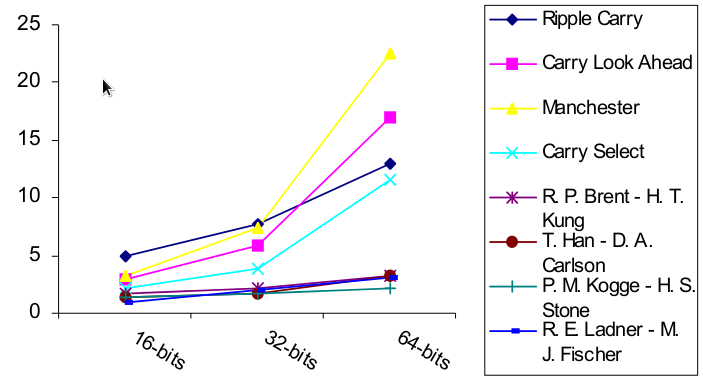
\includegraphics[scale=0.49]{figuras/retardo-bits.png}
\vspace{-5pt}
  \caption{Retardo respecto al tamaño de los operandos}
  \label{retardo-bits}
\vspace{-5pt}
\end{figure}


\begin{figure}[h]
  \centering
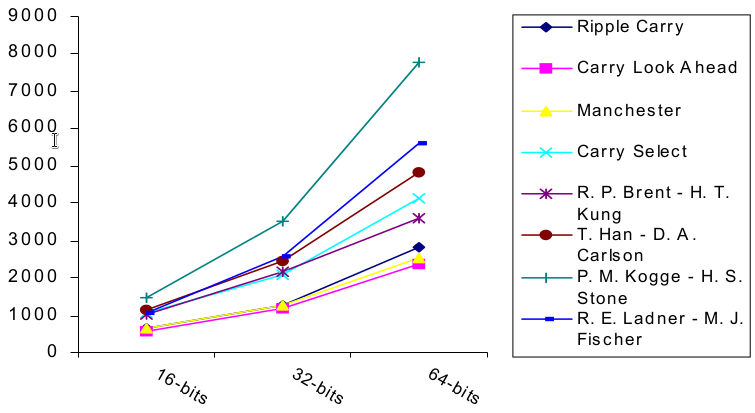
\includegraphics[scale=0.44]{figuras/area-bits.png}
\vspace{-1pt}
  \caption{Área respecto al tamaño de los operandos}
  \label{area-bits}
\vspace{-15pt}
\end{figure}

\begin{table}[h]
\centering
\begin{tabular}{|l|l|l|}
\hline
\multicolumn{1}{|c|}{\textbf{Arquitectura}} & \multicolumn{1}{c|}{\textbf{Retardo Máx.   }} & \multicolumn{1}{c|}{\textbf{Área}} \\ \hline
Ripple Carry  & \(O(n)\) & \(O(n)\) \\ \hline
Carry Look-Ahead  & \(O(\log_2(n))\) & \(O(n\log_2(n))\) \\ \hline
Ladner-Fisher &\( O(\log_2(n))\) & \(O(n\log_2(n))   \) \\ \hline
Sklansky &\( O(\log_2(n))\) & \(O(n\log_2(n))\) \\ \hline
Kogge-Stone & \( O(\log_2(n))\) & \(O(n\log_2n)\)\\ \hline
%Han-Carlson & \( O(\log_2(n))\) &... \\ \hline % Lo quito ya que no encuentro la función de complejidad de área.
Brent-Kung & $O(\log_2(n))$ & \(O(n)\) \\ \hline
\end{tabular}
\caption{Resumen de las funciones de retardo y área de algunos sumadores}\label{tabla:sumadores}
\end{table}

% BKA  Cantidad de operadores (2*n)-2-log_2(n)
% KSA  # de operadores n*log_2(n)-n+1


Resumimos en la tabla \ref{tabla:sumadores} las características y diferencias entre los distintos sumadores\cite{6120598}. Incluimos al \textbf{ripple carry}, por ser la implementación más simple, y al \textbf{carry look-ahead} por ser el sumador que propone el cálculo en paralelo de los acarreos para disminuir logarítmicamente el tiempo de retardo.

%Agregar las referencias a los papers si se puede

%Para justificar la tabla de arriba, vemos los siguientes dos papers:

%"A unified Adder Design" - Wang, Parhi.

%CARACTERIZACIÓN DE SUMADORES EN TECNOLOGÍAS FUERTEMENTE SUBMICRÓNICAS -  Adrián Estrada, Carlos J. Jiménez, Manuel Valencia



\section{Fundamentos teóricos de la suma}
A los fines de poder implementar estos sumadores, desarrollaremos las ecuaciones que nos permitan llegar a la descripción del \cursi{hardware}.

\subsection{Semisumador y sumador completo}
\subsubsection{Semisumador}
El {\bf Semisumador} (Half-adder) recibe 2 bits de entradas \(a\) y \(b\) y produce un bit de suma \(s\) y un bit de acarreo \(c\).

\begin{subequations}
\begin{align}
s &= a \oplus b\\
c &= ab
\end{align}
\end{subequations}

\subsubsection{Sumador Completo}
Luego definimos un Sumador Completo de un bit, o Full Adder:
\begin{center}
\begin{tabular}{lll}
Entradas: & Bits de operandos \(a\) , \(b\) y carry-in \(c_{in}\) & (o \(a_i, b_i, c_i\) para la etapa \(i\)) \\
Salidas: & Suma \(s\) y carry-out \(c_{out}\) & (o \(s_i\) y \(c_{i+1}\) para la etapa \(i\)) \\
\end{tabular}
\end{center}

\begin{subequations}
\begin{align}
s &= a\oplus b \oplus c_{in}
\label{s}
\\
c_{out}&= a b + a c_{in} + b c_{in}
\label{c}
\end{align}
\end{subequations}
%\(c_{out}= (a\wedge b )\vee (a \wedge c_{in}) \vee (b\wedge c_{in})\)

Podemos construir un {\bf sumador completo} (full-adder) combinando las ecuaciones del sumador y semisumador, como vemos en la figura \ref{fig:fulladder}:

\vspace{-1pt}

\begin{figure}[h]
  \centering
\hspace{-23pt}
\begin{subfigure}[b]{0.3\textwidth}
                \centering
                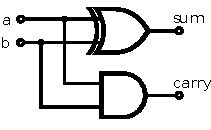
\includegraphics[width=\textwidth]{figuras/halfadd_schem.pdf}
                \caption{Semisumador}
                \label{fig:halfadder}
        \end{subfigure}
\begin{subfigure}[b]{0.5\textwidth}
                \centering
                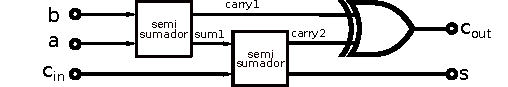
\includegraphics[scale=1.3]{figuras/fullAdd_schem.pdf}
                \caption{Sumador completo}
                \label{fig:fulladder}
        \end{subfigure}

  \caption{Bit adders}\label{fig:bitadders}

\end{figure}

\vspace{0.5cm}

%\section{Selección de la arquitectura del sumador}
%Proponemos el uso de Celdas estándard CMOS (Complementary Metal Oxide Silicon) para la implementación\footnote{Para ver otras posibilidades de implementación lógica, ver (FALTA CITA) RABAEY}. El carácter de nuestro flujo de diseño así lo requiere, ya que se utilizarán herramientas de síntesis de circuitos digitales basadas en celdas estándars. Quedan entonces descartadas las implementaciones utilizando transmition gates, lógica dinámica u otro tipo de implementacion lógica.

\subsubsection{Ripple Carry Adder}

Definimos el sumador Ripple Carry Adder (RCA), utilizando \(n\) sumadores completos para sumar 2 operandos de \(n\) bits. El sumador de \(n\) bits produce una salida de \(n\) bits y una salida de acarreo \(c_{out}\).

Este sumador se implementa conectando como muestra la figura \ref{fig:RCA} el bloque \verb.fullAdd. (Sumador Completo). El camino crítico de la señal se determina considerando el peor camino de propagación de la señal.  

%\vspace{-1pt}
\begin{figure}[h]
  \centering
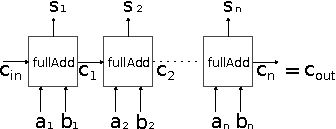
\includegraphics[scale=1.5]{figuras/binnaryAdder.pdf}
  \caption{Ripple Carry Adder}
  \label{fig:RCA}
\end{figure}

El retardo del camino crítico de un sumador de $n$ bits es:

\begin{equation}
T_{RCA} = (n-1)T_m+ T_{FA}
\end{equation}

Siendo $T_m$ el retardo del circuito de generación del acarreo de un sumador completo y $T_{FA}$ el retardo de un sumador completo. Es decir, el retardo es proporcional al tamaño de los operandos.

%\cite{estrada-gimenez}
%Comenzamos con el RCA (Ripple Carry Adder), que tiene un área O(n) y un retardo de compuerta (Delay) de O(n).
%Luego tenemos al CLA (Carry Look-Ahead Adder) con un área de O(n*log(n)) y un delay de O(log(n)).
%Carry Skip Adder(CSA)
%Carry Increment Adder (CIA) Área O(n) y Delay O (nl + 2/ l +1 )  
%Carry Select Adder (CSelA)Área O(n) y Delay O (nl + 2/ l +1 ) 
 
% El delay de un RCA está en pag. 77 de Computer Arithmetic de Behrooz Parhami

\subsection{Sumadores \cursi{carry lookahead}}

La clave para sumar rápido es plantear el problema de la suma como el problema de generar las señales de acarreo en el menor tiempo posible; eso queda evidenciado al interpretar la ecuación \ref{s_i}. Por lo tanto, el objetivo será lograr un bloque generador de las señales de acarreo de baja latencia\cite{arithmeticComputer}.
%Pag. 85 - Section 5.6 (ver como se cita en latex la página)

Ya que una vez que el acarreo en la posición \(i\) es conocido, se puede calcular la suma como:
\begin{equation}\label{s_i}
s_i = a_i \oplus b_i\oplus c_i
\end{equation}

Con respecto al acarreo, lo importante es si en una posición dada el acarreo se \emph{genera} ó se \emph{propaga}. Con las siguientes ecuaciones lógicas podemos definir esas señales:
%

%\vee es el OR
%\wedge es el AND
%\oplus es el XOR
%$$a_i=\lnot{a_i}\wedge\lnot{b_i}=\lnot{(a_i \vee b_i)}$$
$$g_i=a_ib_i$$
$$p_i=a_i \oplus b_i$$


Asumiendo que estas señales se han calculado y están disponibles, podemos calcular recursivamente el acarreo de la siguiente forma:
\begin{equation}
%c_{i+1}=g_i\vee (c_i \wedge p_i)
c_{i+1}=g_i + c_i p_i
\end{equation}


\noindent Esto quiere decir que un acarreo entrará en la etapa \(i+1\) si éste se genera en la etapa \(i\), o si entra en la etapa \(i\) y se propaga.

\subsection{Desenrollando la recurrencia del acarreo}
Uno puede desenrollar esta fórmula recursiva del acarreo hasta lograr una función que dependa directamente de los operandos ($a$ y $b$) y del acarreo de entrada $c_{\text{in}}$:
\begin{equation}
\begin{align}
c_i &= g_{i-1} + p_{i-1}c_{i-1}\notag\\
&=g_{i-1}+p_{i-1}(g_{i-2}+p_{i-2}c_{i-2})=g_{i-1}+p_{i-1}g_{i-2}+p_{i-1}p_{i-2}c_{i-2}\notag\\
&=g_{i-1} + p_{i-1}g_{i-2}+p_{i-1}p_{i-2}g_{i-3}+p_{i-1}p_{i-2}p_{i-3}c_{i-3}\notag\\
&=g_{i-1} +p_{i-1}g_{i-2}+p_{i-1}p_{i-2}g_{i-3}+p_{i-1}p_{i-2}p_{i-3}g_{i-4}+p_{i-1}p_{i-2}p_{i-3}p_{i-4}c_{i-4}\label{gyp}	
\end{align}
\end{equation}

El proceso se repite hasta que el último término contenga $c_0 = c_{\text{in}}$. Podemos computar todos los acarreos en un sumador de $k$-bit directamente con las señales auxiliares ($g_i,p_i$) y $c_{\text{in}}$, utilizando compuertas lógicas AND-OR con un fan-in máximo de $k+1$. Para $k=4$, tenemos:
\begin{equation}
\begin{align}
c_4 &=g_{3} +p_{3}g_{2}+p_{3}p_{2}g_{1}+p_{3}p_{2}p_{1}g_{0}+p_{3}p_{2}p_{1}p_{0}c_{0}\\
c_3 &=g_{2} +p_{2}g_{1}+p_{2}p_{1}g_{0}+p_2p_1p_0c_0\\
c_2 &=g_{1} +p_{1}g_{0}+p_{1}p_{0}c_{0}\\
c_1 &=g_0+p_0c_0\\
\label{carries}	
\end{align}
\end{equation}	
Aquí, $c_4$ y $c_0$ son los $c_{\text{out}}$ y $c_{\text{in}}$ respectivamente de un sumador de 4-bits. Podemos usar un bloque de acarreo basado en estas ecuaciones, y usando compuertas AND de 2 entradas para $g_i$ y compuertas XOR de 2 entradas para $p_i$ y los bits de suma, construimos un sumador de 4-bits. Este sumador es conocido como \emph{carry lookahead adder (CLA)}. Notar que como $c_4$ no se usa para calcular la suma, no es necesario aplicar la ecuación \ref{carries} y lo podemos obtener usando una ecuación más simple, sin tener casi un deterioro en velocidad:
\begin{equation}
\begin{align}
c_4 = g_3 + c_3p_3 \notag
\end{align}
\end{equation}
La red de acarreo que resulta de estas ecuaciones la podemos ver en la figura \ref{cla4bits}.
\begin{figure}[h]
  \centering
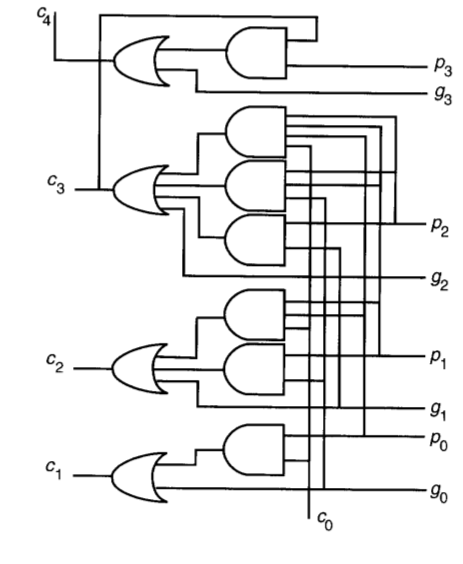
\includegraphics[scale=0.43]{figuras/fulladder4bitcla.png}
\vspace{-1pt}
  \caption{CLA 4-bits}
  \label{cla4bits}
\vspace{-15pt}
\end{figure}

Si observamos las ecuaciones \ref{carries}, vemos que el retardo de esta red será el retardo $T_{AND_n}$ de la mayor celda AND, mas el retardo $T_{OR_n}$ de la operación OR de $n$ entradas. Esto es un inconveniente, ya que según aumenta el fan-in también aumenta el retardo. El retardo de un sumador construido con esta red tendrá también el retardo $T_p$ del cálculo de $p$ mas el retardo de un sumador completo.
\begin{equation}
T_{CLA} = T_p + T_{AND_n} + T_{OR_n} + T_{FA}
\end{equation}

Se pueden realizar por medio de árboles binarios una reducción a celdas con un fan-in de dos (por ejemplo), pero agregando una etapa por cada reducción, en ese caso el retardo en este circuito sería en función del $\log_2 n$.


% INTERESANTE: Clock periods in contemporary microprocessors are rather short; they are shorter than 10 times the delay of a full-adder.

\subsection{Sumadores de Prefijo Paralelos (\emph{Parallel Prefix Adders})}
En la sección anterior vimos como desarrollar ecuaciones que nos permiten obtener las señales de acarreo a partir de las señales auxiliares, para poder calcular la suma del bit $n$, sin esperar a que el acarreo del bit $n-1$ sea computado. Aunque esta solución tal cuál como la presentamos deja de ser aplicable según aumenta $n$, nos permite abordar \textbf{el problema del cálculo de los acarreos como un problema de prefijo paralelo}.
\subsubsection{Problema de prefijo paralelo (\emph{parallel prefix problem})}\label{subsec:prefixProblem}
El problema de prefijo paralelo es:

\begin{equation}
\begin{align}
\text{Dado:}\\
 & \text{Entradas:} x_0,x_1,\dotsc,x_{k-1} \\
 & \text{Un operador + asociativo}\\ 
\text{Computar}:&x_0 \nonumber \\
&x_0+x_1 \nonumber \\ 
&x_0+x_1+x_2+ \nonumber \\ 
&\vdots \nonumber \\ 
&x_0+x_1+x_2+\dotsb+x_{k-1} \nonumber
\end{align}
\end{equation}

\subsubsection{Cómputo del acarreo como un problema de prefijo paralelo}
Pensemos la ecuación \ref{gyp} de la siguiente forma, asumiendo que $c_0=c_\text{in}$ viene desde otro bloque:
\begin{equation}
\begin{align}
g_{[i,i+3]} &= g_{i+3}+g_{i+2}p_{i+3}+g_{i+1}p_{i+2}p_{i+3}+g_{i}p_{i+1}p_{i+2}p_{i+3}\nonumber\\
p_{[i,i+3]} &= p_{i}p_{i+1}p_{i+2}p_{i+3}\nonumber
\end{align}
\end{equation}

Podemos interpretar estas ecuaciones de la siguiente forma: las cuatro posiciones de bits propagan colectivamente un acarreo $c_\text{in}$ si y solo sí cada una de las posiciones propaga; y el bloque gener	a un acarreo si en la posición $i+3$ se genera uno, o se podrouce en la posición $i+2$ y es propagado por la posición $i+3$, etc.

Con este procedimiento podemos llegar a expresar una generalización muy importante, para bloques adyacentes que se superponen $[i_1,j_i]$ y $[i_0,j_0]$, con $i_0 \leq i_1 - 1 \leq j_0 < j_i $:
\begin{equation}
\begin{align}
g_{[i_0,j_1]} &= g_{[i_1,j_1]}+g_{[i_0,j_0]}p_{[i_1,j_1]} \nonumber\\
p_{[i_0,i_1]} &= p_{[i_0,j_0]}p_{[i_1,j_1]}\nonumber
\end{align}
\end{equation}
Aquí, $g_{[i_0,j_1]}$ y $p_{[i_0,i_1]}$ son las señales que producimos de 2 bloques adyacentes ($B''$ y $B'$ con sus señales asociadas $(g'',p'')$ y $(g',p')$) que para simplificar la notación nos permite reescribir la anterior ecuación como:
\begin{equation}
\begin{align}
g &= g'' + g'p''\nonumber\\
p &= p'p''\nonumber
\end{align}
\end{equation}
Ahora entonces definimos un operador acarreo $\circ$ para condensar estas operaciones:
\begin{equation}
\begin{align}
(g,p) &= (g'',p'') \circ (g',p') = (g'' + g'p', p'p'')\nonumber
\end{align}
\end{equation}
Este operador es un operador asociativo, y esto se puede demostrar utilizando la propiedad asociativa de los operadores OR y AND. Finalmente, ya tenemos un operador asociativo, y las entradas $(g''',p''')$,$(g'',p'')$,$(g',p'),\ldots$ que nos permiten plantear el problema de la construcción de la red (o bloque) de acarreos, como un \emph{problema de prefijo paralelo}:
\begin{equation}\label{eq:ppProblem}
\begin{align}
\text{Dados:}\\
 & \text{Entradas:} (g_0,p_0),(g_1,p_1),\dotsc,(g_{k-1},p_{k-1}) \\
 & \text{Un operador} \circ \text{asociativo}\\ 
\text{Computar}:\\
(G_0,P_0) = &(g_{[0,0]},p_{[0,0]})\\
(G_1,P_1) = &(g_{[0,0]},p_{[0,0]})\circ(g_{[0,1]},p_{[0,1]})\\
&\vdots  \\
(G_{k-1},P_{k-1}) = &(g_{[0,0]},p_{[0,0]})\circ(g_{[0,1]},p_{[0,1]})\circ \dotsc \circ(g_{[0,k-2]},p_{[0,k-2]})\circ(g_{[0,k-1]},p_{[0,k-1]})
\end{align}
\end{equation}
Retomando la ecuación \ref{s_i} de la suma, y con estas ecuaciones que nos dan las señales propagadas o generadas del acarreo, podemos construir distintos sumadores, que varían en la red de cálculo del acarreo, particularmente en cómo se elija la asociación del operador \cursi{acarreo} (a veces también mencionado como \cursi{operador punto}). La implementación mas básica (y lenta) sería la de ir asociando en serie a este operador, como vemos en la figura \ref{fig:ppserie}. Todos los sumadores de prefijo paralelo se diferencian escencialmente en la forma de asociar.
\begin{figure}[h!]
  \centering
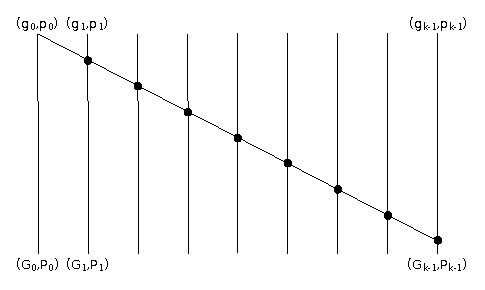
\includegraphics[scale=1.4]{figuras/ppserie.eps}
  \caption{Red de prefijo en serie, una forma gráfica de ver la ecuaciones del cálculo prefijo en \ref{eq:ppProblem}. Notar que cada línea representa dos bits. Los puntos negros representan al operador acarreo.}
\label{fig:ppserie}
%\vspace{-10pt}
\end{figure}
%118 del Parhami " Computer Arithmetic: Algorithms and Hardware Designs."



\subsection {Sumador de Brent-Kung}
Para tener en cuenta el problema de la interconexión entre las compuertas de forma tal que estas sean mínimas y que el área de celdas y de conexión se minimicen, se propone el sumador de Brent-Kung\cite{brent-kung}. Este sumador es una versión que considera el problema de la interconexión entre las compuertas, de una forma que minimice el área, a costa de un aumento en el retardo. Esto se expresa en la función de retardo que es \(2\log_2(n)-2\), a diferencia de los sumadores de Ladner-Fisher\cite{ladner-fischer}, Kugge-Stone\cite{kogge-stone} y Sklansky\cite{sklansky} que en \(\log_2(n)\) etapas calculan todas las señales de acarreo. 


\subsubsection {Operador de Brent-Kung}
El operador $\circ$ se define\footnote{Para respetar la notación de la bibliografía original comenzamos a utilizar la notación lógica con \(\vee\), \(\wedge\) y \(\oplus\) como los operadores booleanos AND, OR y XOR respectivamente} como:
\begin{equation}
(g,p) \circ (\hat{g},\hat{p}) = (g\vee(p\wedge\hat{g}),p\wedge\hat{g})\label{gap}
\end{equation}

\begin{figure}[h!]
  \centering
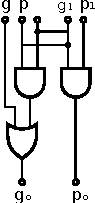
\includegraphics[scale=1.0]{figuras/dotOp_schem.pdf}
%\vspace{-5pt}
  \caption{Operator Punto de Brent-Kung}
  \label{dotOp}
%\vspace{-15pt}
\end{figure}
El operador Punto de Brent-Kung es asociativo, es decir:
$$((a,b) \circ( c,d))\circ (e,f)  = (a,b)\circ((c,d)\circ(e,f))$$
Y por lo tanto podemos ahorrarnos los paréntesis y escribimos:
$$(a,b)\circ(c,d)\circ(e,f)\circ...$$

\subsubsection {Circuito de Generación y Propagación de acarreo}
Ahora necesitamos un circuito que con cada bit de entrada de los operandos \(a\) y \(b\) calcule la señal de acarreo y la de propagación:
$$g_i=a_i \wedge b_i, p_i=a_i\oplus b_i$$
Esas señales se generan en paralelo, dado dos números binarios \(a[n]\) and \(b[n]\) de longitud \(n\).

%vspace{-10pt}

\begin{figure}[h!]
  \centering
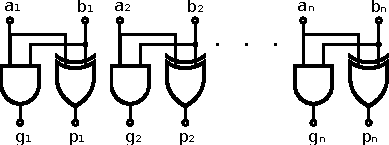
\includegraphics[scale=1]{figuras/gAndPs_schem.pdf}
  \caption{Generación y Propagación del Acarreo}
  \label{gAndPs}
\end{figure}

\subsubsection {Red de Prefijo Paralelo}
\noindent Con la figura \ref{bKung16}, detallamos ahora la red de prefijo paralelo con un fan-out máximo de dos, lo cuál diferencia a el sumador de Brent-Kung de los otros sumadores de prefijo paralelo. La red se realiza con 2 elementos: Los puntos negros son los operadores punto de Brent-Kung de la figura \ref{dotOp} y con buffers (los puntos blancos) que realizan una copia de la señal. Cada cable representa un par de bit \(g_i\),\(p_i\) de la figura \ref{fig:bkungadder}.

\subsubsection {Circuito completo}
Con la red de prefijo paralelo lista, podemos armar el circuito propuesto en el paper de Brent-Kung\cite{brent-kung}. A los fines de la implementación en HDL, mostramos el circuito visto de una forma alternativa en la figura \ref{fig:bkungadder}. Pero aprovechamos la oportunidad para generalizar un poco este resultado. Si retomamos la definición de la suma planteada en la ecuación \ref{s_i}:
$$
s_i = a_i \oplus b_i\oplus c_i
$$
y notamos que en la figura \ref{fig:bkungadder} se calcula $a_i \oplus b_i$, y que con los $G_i$ y los $p_{i-1}$ podemos construir la suma. Por lo tanto, no importa de qué forma se generen estas señales en la red de prefijo paralelo, podemos calcular el valor de $s_i$, como vemos de forma más genérica en la figura \ref{fig:ppadder}.

\begin{figure}[h]
  \centering
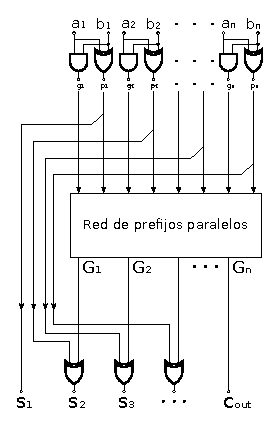
\includegraphics[scale=1.5]{figuras/arquitectura_schem_generico.eps}
  \caption{Sumador de prefijo paralelo}
  \label{fig:ppadder}
\end{figure}

\begin{figure}[h!]
\vspace{-5pt}
  \centering
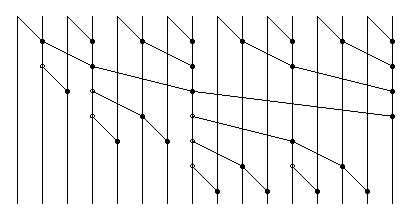
\includegraphics[scale=1.4]{figuras/bKung16.eps}
  \caption{Red de prefijo paralelo para Brent-Kung (ejemplo de 16 bits)}
\label{bKung16}
\vspace{-10pt}
\end{figure}

\begin{figure}[h]
  \centering
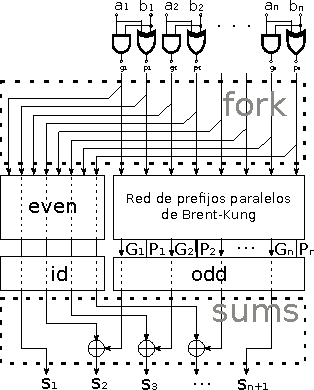
\includegraphics[scale=1.5]{figuras/arquitectura_schem.pdf}
  \caption{Sumador de Brent-Kung}
  \label{fig:bkungadder}
\end{figure}

\subsection{Sumador de Sklansky}\label{subsec:sklansky}
Para realizar este sumador, debemos desarrollar la red de cálculo paralelo de los acarreos, a la forma propuesta por Skalansky. Esta forma se conoce como \emph{divide and conquer}, y la evidenciamos con un ejemplo para sumandos de 16 bits en la figura \ref{fig:sklansky16}. Los puntos negros representan el operador punto (definido anteriormente como el operador de Brent-Kung), notar que tiene menos cantidad de etapas de operaciones (en proporción de $\log_2(n))$) por lo tanto es un sumador más rápido que el de Brent-Kung, pero hay nodos que tienen un fan-out de hasta $\frac{n}{2}$, lo cuál resulta en mayor capacidades parásitas, haciendo más lento el circuito en ese nodo.

\begin{figure}[h!]
\vspace{-5pt}
  \centering
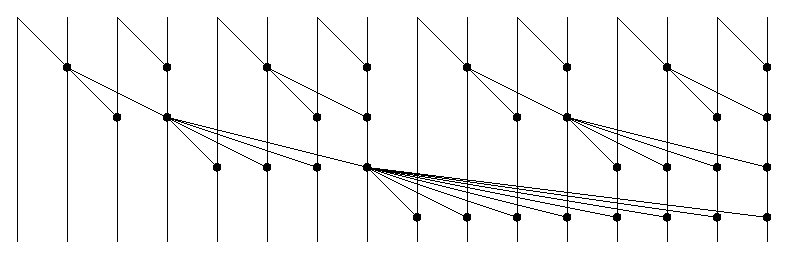
\includegraphics[scale=0.7]{figuras/sklansky16.eps}
  \caption{Red de prefijo paralelo para Sklansky (ejemplo de 16 bits)}
\label{fig:sklansky16}
\vspace{-10pt}
\end{figure}

\backmatter


%%%%%%%%%%%%%%%%%% CONFIGURACION DE CABECERA %%%%%%%%%%%%%%%%%%%%%%%%%%%%%%%%%%%%%%
\pagestyle{fancyplain}                                                            %
%%%Formato partes
\renewcommand{\partname}{PARTE}
%%%Formato capítulo: N.Nombre                                                     %
\renewcommand{\chaptermark}[1]{\markboth{\textbf{\small{CAPÍTULO \thechapter}}}{}}%
%%%Formato sección: N.M.Nombre                                                    %
\renewcommand{\sectionmark}[1]{\markright{\textbf{\small{\thesection. #1}}}}      %
%%%%%%%%%%%%%%%%%%%%%%%%%%%%%%%%%%%%%%%%%%%%%%%%%%%%%%%%%%%%%%%%%%%%%%%%%%%%%%%%%%%

\bibliographystyle{classes/CUEDbiblio} % Title is link if provided 
%\bibliographystyle{IEEEtran.bst}
\bibliography{pruebabib}


%\nocite{jitter2,jitter3}
\listoffigures 
\listoftables 

\end{document}
